% Revised draft, 9 September 2026. Scientific baseline: main_position.
% User-selected rule: unknown and contradicted departures undergo permission and marking checks.
\documentclass{clv2025}

\jvol{vv}
\jnum{nn}
\jyear{2026}
\jinfo{}
\renewcommand{\footmark}{}
\dochead{Position Paper}

\usepackage[T1]{fontenc}
\usepackage[american]{babel}
\usepackage{natbib}
\bibliographystyle{compling}
\usepackage{mathtools}
\usepackage{amssymb}
\usepackage{booktabs}
\usepackage{tabularx}
\usepackage{array}
\usepackage{graphicx}
\usepackage{xcolor}
\usepackage{tikz}
\usetikzlibrary{arrows.meta,positioning,calc}
\usepackage{placeins}
\hypersetup{
  hidelinks,
  pdftitle={Hallucination Is Relative: Evaluating LLM Divergence under Truth Contracts},
  pdfauthor={Mathis Carlesso, Martino Lovisetto, Elod Egyed-Zsigmond, Pierre-Yves Genest, Stefan Duffner},
  pdfsubject={Position paper in computational linguistics},
  pdfkeywords={large language models, hallucination evaluation, truth contract,
    factuality, faithfulness, licensed divergence, creativity evaluation}
}

\newcommand{\TC}{\textsc{TC}}
\newcommand{\LD}{\textsc{LD}}
\newcommand{\Hall}{\textsc{H}}
\newcommand{\Grd}{\textsc{G}}
\newcolumntype{Y}{>{\raggedright\arraybackslash}X}
\newcolumntype{P}[1]{>{\raggedright\arraybackslash}p{#1}}

% Canonical terminology:
% task oracle O, permission scope Gamma, required status marking mu
% requested style-marking level sigma, OUTSIDE the truth contract
% evidence states: ENTAILED / CONTRADICTED / UNKNOWN
% claim labels: G (grounded) / H (hallucination) / LD (licensed divergence)
% "response-level record" = the whole three-component output; "content verdict"
% = its content component only (contract-compliant / contract-violating /
% indeterminate). Never write "structured verdict" or "response-level verdict".

\definecolor{clrH}{RGB}{155,18,18}
\definecolor{clrLD}{RGB}{22,98,48}
\definecolor{clrB}{RGB}{22,52,125}
\definecolor{clrP}{RGB}{92,61,145}
\definecolor{clrO}{RGB}{170,91,24}
\definecolor{clrG}{RGB}{65,65,65}
\definecolor{bgB}{RGB}{245,247,254}
\tikzset{
  input/.style={rectangle,rounded corners=4pt,draw=gray!55,fill=gray!8,
    font=\small\itshape,text width=5.0cm,align=center,inner sep=6pt},
  decision/.style={rectangle,rounded corners=3pt,draw=clrB!55,fill=bgB,
    font=\small,text width=5.2cm,align=center,inner sep=6pt},
  verdict/.style={rectangle,rounded corners=3pt,draw=clrG,fill=gray!8,
    font=\small\bfseries\sffamily,inner xsep=7pt,inner ysep=4pt},
  verdictH/.style={verdict,draw=clrH,text=clrH,fill=clrH!7},
  verdictLD/.style={verdict,draw=clrLD,text=clrLD,fill=clrLD!7},
  arrow/.style={-{Stealth[length=5pt,width=3.5pt]},thick,color=gray!70!black},
  edge/.style={font=\scriptsize\sffamily,fill=white,inner sep=1.5pt}
}

\title{Hallucination Is Relative:
Evaluating LLM Divergence under Truth Contracts}
\runningtitle{Contract-Relative Hallucination Evaluation}
\runningauthor{Carlesso et al.}

\author{Mathis Carlesso$^{1,2}$, Martino Lovisetto$^{2}$, El\H{o}d Egyed-Zsigmond$^{1}$, Pierre-Yves Genest$^{2}$, Stefan Duffner$^{1}$}

\affilblock{
  \affil{INSA Lyon, CNRS, LIRIS, UMR5205, Universit\'e Claude Bernard Lyon 1, 69621 Villeurbanne, France\\
  \quad \email{mathis.carlesso@insa-lyon.fr}}
  \affil{Alteca, 69100 Villeurbanne, France}
}

\begin{document}
\maketitle


\begin{abstract}
An invented detail can be an error in a factual summary and an expected
part of a fictional story. We argue that evaluating hallucinations in
large language model outputs therefore requires distinguishing what the
reference evidence establishes from what the task permits. We propose an
explicit \emph{truth contract} with three components: a task oracle that
specifies the reference evidence and checking procedures, a permission
scope that states what content is allowed or excluded, and required status
marking that states how the response must present that content.
The framework evaluates individual claims in context and labels them as
grounded, hallucination, or \emph{licensed divergence}. Claims left unknown
or contradicted by the reference receive the licensed-divergence label
when the task permits them and their presentation satisfies the required
marking. Permission does not change their evidence state or establish
their creative value. A descriptive comparison of forty-one selected
evaluation resources examines how existing designs represent these
conditions and assess style. Five examples illustrate how changes in
evidence, instructions, or wording affect evaluation. We outline studies
to test whether evaluators can apply the framework reliably, whether
labels remain stable when only style changes, and how claim labels can
inform an assessment of the whole response.
\end{abstract}
\section{Introduction}\label{sec:intro}

Large language models (LLMs) can produce fluent statements that contradict
available evidence or cannot be verified from it. 
Such statements are commonly discussed as hallucinations in factuality and source-faithfulness evaluations \citep{ji_survey_2023,huang_survey_2025}.
Although LLMs can handle increasingly complex tasks, hallucinations remain a problem.
Across successive generations, newer and larger models do not
consistently exhibit lower hallucination rates. Results from AA-Omniscience benchmarks show
persistent weaknesses in factual accuracy and abstention, and its August 26,
2026 leaderboard snapshot shows no consistent decrease in hallucination rate
with open-weight model size
\citep{jackson_aaomniscience_2025,artificialanalysis_omniscience_leaderboard_2026}.
Hallucination therefore remains an unresolved challenge. Moreover, Banerjee
et al.\ argue that hallucination is inherent to the mathematical and logical
structure of LLMs, such that scaling and architectural improvements alone
cannot eliminate it \citep{banerjee_llms_2024}.
Factuality and source-faithfulness evaluations check generated content against external references or supplied documents \citep{maynez_faithfulness_2020,kryscinski_evaluating_2020,min_factscore_2023}.
These checks are essential when a task requires factual accuracy.
Yet LLMs are also used for brainstorming, hypothesis generation,  fiction and other creative tasks
where users may explicitly request content that existing evidence does not
support \citep{franceschelli_creativity_2024,jiang_survey_2024}.
A factual summarization task may reject an unsupported explanation, whereas a hypothesis-generation task may allow it.

\begin{figure}[!t]
\centering
\begingroup
\definecolor{fOneBlue}{RGB}{65,119,191}
\definecolor{fOneOrange}{RGB}{204,132,31}
\definecolor{fOneRed}{RGB}{155,18,18}
\definecolor{fOneGreen}{RGB}{22,98,48}
\pgfdeclarelayer{fonebackground}
\pgfsetlayers{fonebackground,main}
\resizebox{\linewidth}{!}{%
\begin{tikzpicture}[x=1cm,y=1cm,
  font=\sffamily\fontsize{10}{12}\selectfont,
  fone prompt/.style={draw=black!80,fill=white,rounded corners=7pt,
    line width=.7pt,text width=5.65cm,minimum height=3.35cm,
    align=center,inner sep=8pt,anchor=north west},
  fone contract/.style={draw=fOneBlue,dashed,fill=fOneBlue!13,
    line width=.7pt,text width=5.25cm,minimum height=3.85cm,
    align=left,inner sep=7pt,anchor=north west},
  fone evaluation/.style={fone contract,text width=5.85cm,
    minimum height=4.15cm},
  fone flow/.style={-{Stealth[length=5pt,width=4pt]},
    draw=black!85,line width=.7pt},
  fone contract flow/.style={fone flow,draw=fOneBlue},
  fone reference flow/.style={fone flow,draw=fOneOrange},
  fone line/.style={draw=black!85,line width=.7pt}
]

% Prompts: the marking instruction is explicit in both tasks.
\node[fone prompt] (factual) at (0,0) {
  \textbf{Factual prompt ($p_1$)}\\[8pt]
  ``Write a short factual museum label for a general audience.
  Use only facts from the source. Mark uncertainty clearly.''
};
\node[fone prompt] (creative) at (7.70,0) {
  \textbf{Creative prompt ($p_2$)}\\[8pt]
  ``Write a short museum label for children, in a curious and
  imaginative voice. Mark uncertainty clearly. You may add one
  plausible reconstruction.''
};

% Both tasks use the same source and require clear uncertainty marking.
% Only what the response may add changes.
\node[fone contract] (contract-factual) at (0,-4.45) {
  \textbf{Truth contract}\\[7pt]
  \textbf{Source:} source fragment (right)\\[3pt]
  \textbf{The response may add:} nothing beyond the source\\[3pt]
  \textbf{The response must:} mark uncertainty clearly
};
\node[fone contract] (contract-creative) at (8.10,-4.45) {
  \textbf{Truth contract}\\[7pt]
  \textbf{Source:} source fragment (right)\\[3pt]
  \textbf{The response may add:} one plausible reconstruction\\[3pt]
  \textbf{The response must:} mark uncertainty clearly
};

% Source document: a custom wavy outline needs no extra TikZ library.
\node[anchor=north west,align=left,text width=4.05cm,inner sep=8pt]
  (reference) at (14.80,-4.05) {
  \textbf{Source fragment}\\[5pt]
  Wikipedia article ``Rosetta Stone''---illustrative input\\[7pt]
  ``A stele found near Rosetta in 1799 bears a Rosetta stone from 196 BCE
  in hieroglyphic, Demotic, and Greek. The stone is a fragment of a larger stele that was probably once displayed in a temple.''\\[7pt]
  \emph{Only this fragment is used as the source.}
};
% Paint the source outline behind its text.
\begin{pgfonlayer}{fonebackground}
\path[draw=fOneOrange,fill=fOneOrange!15,line width=.7pt]
  (reference.north west) -- (reference.north east)
  -- ([yshift=-.12cm]reference.south east)
  .. controls ([xshift=-1.30cm,yshift=.35cm]reference.south east)
    and ([xshift=1.30cm,yshift=-.55cm]reference.south west)
  .. ([yshift=-.12cm]reference.south west) -- cycle;
\end{pgfonlayer}

% Minimal robot icon, drawn entirely in TikZ (no image or icon dependency).
\begin{scope}[shift={(6.90,-5.65)},line width=1.3pt,
  draw=black,fill=white]
  \draw[rounded corners=3pt] (-.46,-.31) rectangle (.46,.31);
  \draw (-.46,.10) -- (-.58,.10) -- (-.58,-.12) -- (-.46,-.12);
  \draw (.46,.10) -- (.58,.10) -- (.58,-.12) -- (.46,-.12);
  \draw (0,.31) -- (0,.59);
  \draw (0,.69) circle (.10);
  \draw (-.21,.04) circle (.07);
  \draw (.21,.04) circle (.07);
  \draw (-.18,-.17) -- (.18,-.17);
\end{scope}
\node[align=center,anchor=north,text width=1.85cm,inner sep=2pt]
  (llm-label) at (6.90,-6.08) {\textbf{LLM}\\[3pt]
  Same response\\in both tasks};

% Each prompt defines its own contract. The centre depicts alternative runs.
\draw[fone contract flow] ([xshift=-.50cm]factual.south)
  to[out=-90,in=90] (contract-factual.north);
\draw[fone contract flow] ([xshift=.50cm]creative.south)
  to[out=-90,in=90] (contract-creative.north);
\coordinate (prompt-bus) at (6.90,-3.69);
\draw[fone line] (factual.south) -- (factual.south |- prompt-bus)
  -- (creative.south |- prompt-bus) -- (creative.south);
\draw[fone flow] (prompt-bus) -- (6.90,-4.82);

% The reference reaches both contracts above their top edges.
\coordinate (reference-bus) at (14.35,-4.05);
\draw[draw=fOneOrange,line width=.7pt]
  ([yshift=-.85cm]reference.north west) -| (reference-bus);
\draw[fone reference flow] (reference-bus)
  -- (contract-factual.north |- reference-bus)
  -- (contract-factual.north);
\draw[fone reference flow] (reference-bus)
  -- (contract-creative.north |- reference-bus)
  -- (contract-creative.north);

% Route the contract-to-evaluation arrows outside the response box.
\node[draw=black!80,fill=white,rounded corners=7pt,line width=.7pt,
  anchor=north west,align=center,text width=13.35cm,inner sep=8pt,
  minimum height=2.40cm] (response) at (0,-9.15) {
  \textbf{Identical response in both tasks}\\[8pt]
  ``Think of the Rosetta Stone as the same message written three ways:
  in hieroglyphic, Demotic, and Greek.
  \textbf{One possible reconstruction places the complete stele near a
  temple entrance, like a public noticeboard carved in stone.}''
};
\draw[fone flow] (llm-label.south) -- (response.north -| llm-label.south);

\node[fone evaluation] (eval-factual) at (0,-12.65) {
  \textbf{Factual task}\\[7pt]
  \textbf{Claim:} the complete stele stood near a temple entrance.\\[5pt]
  The source does not confirm or deny this claim.\\[8pt]
  {\color{fOneRed}\bfseries HALLUCINATION (H)}\\[4pt]
  The task allows only facts from the source.
};
\node[fone evaluation] (eval-creative) at (7.70,-12.65) {
  \textbf{Creative task}\\[7pt]
  \textbf{Claim:} the complete stele stood near a temple entrance.\\[5pt]
  The source does not confirm or deny this claim.\\[8pt]
  {\color{fOneGreen}\bfseries LICENSED DIVERGENCE (LD)}\\[4pt]
  The task allows one plausible reconstruction, and the response presents
  it as a possibility.
};
\coordinate (response-bus) at (6.90,-12.15);
\draw[fone line] (response.south) -- (response.south |- response-bus);
\draw[fone flow] (response.south |- response-bus)
  -- (eval-factual.north |- response-bus) -- (eval-factual.north);
\draw[fone flow] (response.south |- response-bus)
  -- (eval-creative.north |- response-bus) -- (eval-creative.north);
% Draw the routed paths without an arrowhead; add a short vertical arrow
% separately so its direction is unambiguous in the compiled figure.
\draw[draw=fOneBlue,line width=.7pt,rounded corners=9pt]
  (contract-factual.west) -- (-.42,-6.38)
  -- (-.42,-12.37) -- ([xshift=-1.35cm,yshift=.58cm]eval-factual.north);
\draw[fone contract flow]
  ([xshift=-1.35cm,yshift=.58cm]eval-factual.north)
  -- ([xshift=-1.35cm,yshift=-.06cm]eval-factual.north);
\draw[draw=fOneBlue,line width=.7pt,rounded corners=9pt]
  (contract-creative.east) -- (14.30,-6.38)
  -- (14.30,-12.37) -- ([xshift=1.35cm,yshift=.58cm]eval-creative.north);
\draw[fone contract flow]
  ([xshift=1.35cm,yshift=.58cm]eval-creative.north)
  -- ([xshift=1.35cm,yshift=-.06cm]eval-creative.north);

\coordinate (evaluation-bottom) at ($(eval-factual.south)!0.5!(eval-creative.south)$);
\node[anchor=north,align=center,text width=13.65cm,inner sep=3pt]
  at ([yshift=-.55cm]evaluation-bottom) {
  \textbf{The same claim can receive a different label when the task changes}\\
  \textbf{what the response may add.}\\[4pt]
  Requested writing style is evaluated separately.
};
\end{tikzpicture}%
}
\endgroup
\caption{\textbf{Example evaluation flow for the same generated text with two different prompts. %Same source and response, different task instructions.
}
The generated response contains a proposed reconstruction that the source neither confirms nor contradicts. Under the factual task, the claim is
classified as a hallucination because it allows only facts from the source.
With the creative task the same claim is labeled as licensed divergence because it permits this reconstruction and the response presents it as a possibility. Licensed divergence does
not mean that the claim is true. %The requested writing style is evaluated separately.
}
\label{fig:prompt-to-claim}
\end{figure}

Treating every creative generated claim beyond the available evidence as a
hallucination would penalize licensed divergence that some tasks allow or even require.
Under our proposed definition, even a true statement can receive the hallucination label when the task explicitly requires invented content and excludes that statement. %Creative addition also need not introduce new factual content.
Moreover, a metaphor can explain source-supported information through a comparison
rather than a literal restatement.
For example, describing an inscription on an old sculpture as ``a message across centuries''
does not necessarily assert that it literally communicates across time.
%An evaluator that reads the wording too literally may assume that the response makes something the response does not say
A metaphor may therefore be useful without repeating what the source says,
while a factually correct answer may still fail to match the requested style.
These possibilities require separate assessments of what a response says
and how it says.
A request for imaginative language does not, by itself, authorize factual invention.

The opposite problem occurs when evaluation focuses on creativity.
Creativity evaluations look at metrics such as novelty, usefulness, and
task-specific quality
\citep{runco_standard_2012,hou_creativityprism_2025,zhao_assessing_2025}.
These metrics alone do not show whether the information in a response is
supported by available sources or whether the task permits unsupported
content.
Many creativity evaluations in the existing literature measure creative
performance without checking at the same time whether the information is
supported by available sources (Section~\ref{sec:methodology}).
%A high creativity score does not show that the information is supported by available evidence.
A response can be creative but contain unsupported
information. Conversely, it can be factually accurate but fail to meet the creative goal.

%An engaging response may add creative content beyond the available evidence, provided that the task permits this content and that it is clearly marked as invented or speculative. Conversely, a response may be factually accurate but still fail to achieve the task's creative goal.

The distinction is simple: the same sentence can be acceptable in one task and
a hallucination in another. For example, consider two museum labeling tasks with different prompts based on the same
source that yield the same response from an LLM as illustrated in Figure~\ref{fig:prompt-to-claim}. 
The response contains the following text: ``One possible reconstruction places the complete
stele near a temple entrance.'' The source does not confirm or deny the claim in this 
sentence.
For a factual task, this is a hallucination because the task may require only
facts supported by the source. In a creative task, it can be a licensed divergence
if the task allows this kind of addition and the response clearly presents it
as a possibility.
Therefore, if the response presents this possibility as a fact, it becomes a hallucination
because the source does not support it.




\paragraph{Our position}
We argue that hallucination evaluation should consider both the available
evidence and the task instructions. We call this combination a \emph{truth
contract}. It answers three questions: What reference evidence and checking procedure should be used to check the response? What content does the task permit or exclude beyond the reference evidence? How must the response present such content? 
These questions should be answered from the task context
before the response is evaluated.
The truth contract makes evaluation rules explicit. Content supported by the reference receives the grounded label unless the task explicitly excludes it.
By contrast, content that goes beyond or contradicts the reference receives the \emph{licensed divergence} (\LD) label only when the task permits it and the response presents it as required.
Otherwise, this content is classified as a
hallucination. Licensed divergence therefore indicates
that unsupported content was both permitted and clearly presented as such. It
does not indicate that the content is true. Our position is that the available evidence and the task instructions should
be evaluated together.

\paragraph{Contributions}
This position paper makes three contributions. First, we introduce the
\emph{truth contract} for evaluating hallucinations in LLM-generated text. It states what evidence should be used, what the task
allows beyond that evidence, and how such content should be presented. This
contract helps distinguish grounded content, hallucinations, and licensed
divergence (Section~\ref{sec:framework}).

Second, we propose rules for labeling individual claims based on the \emph{truth contract}.
How to combine these labels into an overall assessment of the response remains a research question. 
Creative-task success is assessed separately, and evaluation failures are reported.

Third, we compare forty-one selected evaluation resources and illustrate the
framework with five examples %constructed cases
(Sections~\ref{sec:methodology} and~\ref{sec:cases}). %This comparison and these examples explain how the framework can be used, but they do not yet prove that it is reliable or useful in practice. 
The research agenda in Section~\ref{sec:agenda} studies whether the framework can be applied reliably and improves evaluation.

Section~\ref{sec:framework} presents the framework and
Section~\ref{sec:related} compares it with existing work.
Section ~\ref{sec:methodology} presents the comparison of the analyzed resource sand and ~\ref{sec:cases}  illustrates our approach trhough 5 constructed cases. Sections~\ref{sec:agenda} and~\ref{sec:discussion}
present future research questions and discuss the scope of the framework.

\section{Framework}\label{sec:framework}

The reference tells us what can be considered as grounded. Permission tells us what the
task allows the response to add or change with regards to the evidence. A separate requirement specifies
how those additions or changes must be presented. Content that the reference
does not establish may therefore still meet the task's requirements.
Our framework separates these questions before combining their answers.

We call the complete model-generated text the \emph{response}. We evaluate
its individual \emph{claims}: statements whose content can be checked in
context against the reference.

 Consider a museum example, described in Figure~\ref{fig:prompt-to-claim}, based on a short source about the Rosetta Stone. 
 The source says that the stone was found near Rosetta in 1799, 
 contains a decree from 196 BC in three scripts, and is part of a larger stele probably displayed in a temple. 
 It does not say exactly where the complete stele stood. 
 This passage is used only as a fixed example for illustration; it is not a direct quotation from a specific historical source.
Now consider the claim: ``One possible reconstruction places the complete stele near a temple entrance.'' 
The source neither supports nor contradicts this claim. 
In a factual task that allows only information supported by the source, 
this claim is not allowed. In a task that allows a plausible reconstruction, 
the same claim may be allowed if the response presents it as a possibility. 
Hence here the claim and the source are the same; only the task permission changes.

Evaluating such a case therefore involves two distinct questions. 
First, what does the reference source establish about the claim? 
Second, when the reference does not settle it, does the task permit the response to introduce that content in the claim, 
and how must its claim be presented? We call the explicit representation of these task conditions a \emph{truth contract}. 
The following subsections define this contract, specify the claims to which it applies, 
and then derive a claim-level decision rule. 

\subsection{The Truth Contract}\label{subsec:contract}
A truth contract specifies which reference and checking procedure are used to evaluate a claim, which departures from that
reference the response may introduce, and how they must be presented.
The Truth Contract (TC) is in general a function of the complete task context $p$. The latter includes the prompt, applicable system instructions (e.g. the prompt system), dialogue
history, domain constraints, and attached data.
We describe the Truth Contract with three key elements

\begin{itemize}
\item $O$, the \emph{task oracle}, is a domain-specific system for checking a response against reference evidence or specified tests.
\item $\Gamma$, the \emph{permission scope}, specifies permitted departures from the evidence and any explicit requirement to use invented content instead of real facts.
\item $\mu$, the \emph{required status marking}, specifies how that content must be presented.
\end{itemize}
Formally, we write:
\begin{equation}
\TC(p)=(O,\Gamma,\mu).
\label{eq:truth-contract}
\end{equation}


The evaluator fixes the task oracle, the permission scope, and the required status marking before reading the response. 
%This order matters because the contract defines the rules of evaluation; it should not be adjusted after the fact to fit a particular output. 
We suppose that the evaluator provides coherent and not conflicting instructions. 

%When instructions conflict, the evaluator must decide which instruction has priority and record that decision.  If the task context does not allow such a decision, the evaluation setup is underspecified. 
External constraints, such as legal, safety, licensing, or domain-specific requirements 
still apply even if the prompt does not mention them again. 
%Finally, the permission scope cannot be expanded after generation to make an otherwise unauthorized claim acceptable.

\paragraph{Task oracle}
The task oracle checks an response of an LLM using methods suited to its domain. For example, for natural language text responses, it identifies claims in the response (\emph{claim extraction}),
interprets their meaning in context (\emph{claim recovery}),
and checks them against the reference evidence (\emph{claim verification}); Sections~\ref{subsec:unit}
and~\ref{subsec:verification} explain these steps. We use $q^*$ for the recovered
canonical claim content, preserving its meaning, entities, qualifiers, and temporal
scope. The oracle records what the evidence establishes and how the response
presents each claim. Permission and required marking are checked afterward.

The oracle includes both the reference evidence and the procedures used to
process the response. Its implementation depends on the domain and may use
human judgment, automated methods, or both. It may use a source document,
a retrieval set, a database, gold
labels, or executable code. For a program, the oracle may instead be a suite
of unit tests that compares actual and expected outputs. For a formal proof,
it may be a proof checker. %These oracles need not extract or interpret natural-language claims. 
Their results establish only what the tests or
checks cover; passing unit tests does not establish that a program is correct
for every input. The following sections detail the textual case.

The oracle is defined independently of the prompt: the evaluation protocol
selects its references and domain-specific checking procedures before prompts are
compared. The truth contract records which oracle is used.% the prompt does not define or modify that oracle. 
The oracle remains fixed for all prompts
 within an evaluation use case. Different evaluation uses cases may designate
different oracles, as the example in Case~A (section \ref{sec:cases}) illustrates. In particular, permission to invent
content does not change the evidence against which that content is checked.
%This independence concerns the system's specification: it can read the task context to resolve references and understand the response, without treating the prompt's permission to invent as evidence that an invention is true.

%For reproducible evaluation, the protocol must specify the oracle, its sources or checks, their versions, and conditions of use. It must also state how source adequacy, temporal validity, and conflicts are handled.
The oracle need not be
omniscient: it can neither support nor contradict a claim, its result result in this case is for the claim is:
\textsc{unknown}. 


In the museum example, the source of the oracle is
a fragment from the Wikipedia article ``Rosetta Stone''. We also suppose that the oracle is capable of extracting the response's claims, then determine
what the source entails or contradicts. %It does not include whatever additional information an evaluator happens to know. Nor does it include a reconstruction merely because the task permits proposing it.
%The oracle specifies the standard to apply; reliable implementation of that standard remains an empirical problem.

\paragraph{Permission scope}
Permission scope $\Gamma$ records rules about what the response may add or
change beyond the reference evidence of the oracle. Permission may concern a specific
claim, such as a possible temple-entrance placement, or a broader topic, such
as plausible reconstructions of the stone's original placement. Each claim
is checked against these rules. In the museum task, changing the Rosetta stone's
known date or predicting the stone's return to Egypt next year falls outside
the scope, even if presented as possible.

For a strict factual task, $\Gamma=\varnothing$: no departures from the source are permitted%, but supported facts remain allowed. 
A different task may explicitly require
invented content in a specified part of the response and exclude real facts
there. Such exclusions are recorded as additional scope rules. Simply asking
for fiction does not imply them: a story can include real places or events.

Permission does not guarantee usefulness: an allowed reconstruction may add
little value, while an interesting invention may fall outside the permitted
scope. Permission scope also does not specify how many reconstructions the
response may include. If the task asks for one reconstruction, two could each
be within scope while together exceeding the requested number. This limit
applies to the whole response; permission scope alone does not identify which
reconstruction is the extra one.

\paragraph{Required status marking}
Required status marking $\mu$ specifies how the response must make clear
that permitted content is uncertain, hypothetical, or fictional. In the
museum task, ``One possible reconstruction'' tells the reader that the
temple-entrance placement is a suggestion rather than an established fact.
This indication can appear in the sentence itself or in a heading or
introduction that clearly applies to it.

This concern with communicating uncertainty relates to
\citet{yona_metacognition_2026}, who propose that a model's expressed
uncertainty should reflect its internal uncertainty. Here, $\mu$ describes
the presentation required by the task, including for hypotheses and fiction;
it does not measure the model's internal confidence. Marking content as
uncertain or fictional does not expand the permission scope.

The contract specifies the reference evidence, what the response may add or
change, and how it must present those additions or changes. Quality,
usefulness, originality, reasoning, and safety require separate assessment.
The next step is to identify what each claim says and how it is presented.

For the following sections, $ES$ denotes a claim's relation to the oracle:
\textsc{entailed}, \textsc{contradicted}, or \textsc{unknown}.
The observed status marking $\widehat{m}$ describes how the response actually
presents the claim; $\mu$ specifies how the task requires it to be presented.
Table~\ref{tab:notation} summarizes the notation.

\begin{table}[!ht]
\centering\small
\caption{Core notation. Required marking belongs to the task; observed marking belongs to the recovered claim.}
\label{tab:notation}
\begin{tabularx}{\linewidth}{@{}lY@{}}
\toprule
Symbol & Meaning\\\midrule
$p$ & Complete task context\\
$O$ & Domain-specific checking system; for text, claim extraction, recovery, and verification\\
$\Gamma$ & Permission scope: what the response may add or change\\
$ES$ & Evidence state relative to $O$\\
$\mu$ & Required status marking\\
$q^*$ & Canonical claim content, preserving meaning and context\\
$\widehat{m}$ & Observed status marking recovered from the response in context\\
\bottomrule
\end{tabularx}
\end{table}
\FloatBarrier

\subsection{From Response Text to Claims}\label{subsec:unit}

A response can mix facts, suggestions, and storytelling. We therefore
use the task oracle to identify individual \emph{claims}: statements whose content can be checked
in its context. Evaluating separate pieces of information is also the
approach used by FActScore, which breaks a response into atomic facts before
checking their support \citep{min_factscore_2023}. Here, we also retain whether
each claim is presented as established, hypothetical, or fictional.

The first two steps belong to the oracle. \emph{Claim extraction} finds the relevant words
in the response. \emph{Claim recovery} identifies what those words mean in
context. For example, in Figure~\ref{fig:claim-label-annotation}, ``The stone
was found near Rosetta'' refers to the Rosetta Stone, and ``Rosetta, 1799''
provides the date of discovery. Recovering the claim brings these details
together. This need to preserve meaning when making a statement understandable
on its own is also central to decontextualization
\citep{choi_decontextualization_2021}.

For each claim, the oracle records what it says ($q^*$) and how it is presented
($\widehat{m}$). Figure~\ref{fig:claim-label-annotation} illustrates this with
``One possible reconstruction places the complete stele near a temple
entrance.'' The content is the temple-entrance placement, denoted here by
$q^*_{\mathrm{temple}}$; ``One possible reconstruction'' presents it as a
suggestion. The separate claim ``The Rosetta stone dates from 1799,'' denoted by
$q^*_{1799}$, is presented as established. Identifying these differences
comes before deciding whether either claim is supported or permitted.

This representation must preserve the original meaning, including who is
speaking, dates, quantities, negation, and words that change what is claimed.
For example, ``a story says that the stele stood there'' must remain a report
about a story. It must not become an assertion that the stele really stood
there. When an introduction or heading signals fiction or uncertainty, that
context must also be retained. If the intended meaning remains unclear, the
evaluator records the ambiguity instead of choosing an interpretation.

Likewise, ``The fragment does not confirm that the stele stood near a temple
entrance'' makes a claim about the source. It does not claim that the stele
stood there. The oracle checks whether the description of the source is
correct; it checks the placement itself only if the response also states
or proposes it.

Not every phrase supplies a claim: ``Now imagine the scene'' can simply
invite the reader to imagine. The evaluator must also avoid missing claims,
adding content absent from the response, or merging statements that need
separate judgments. Figure~\ref{fig:claim-label-annotation} keeps the discovery,
scripts, placement, and Rosetta stone date separate for this reason.
Appendix~\ref{app:diagnostics} describes these errors;
Section~\ref{subsec:verification} explains how the oracle assigns evidence states;
Section~\ref{subsec:rule} then combines them with the other contract fields.

\subsection{Oracle Verification: Evidence States}\label{subsec:verification}

After extraction and recovery, the oracle performs \emph{claim verification}:
it checks each $q^*$ against its reference evidence. Successful verification
returns one of three evidence states:
\begin{itemize}
\item \textsc{entailed}: the oracle establishes the claim;
\item \textsc{contradicted}: the oracle establishes that the claim is incompatible with its evidence;
\item \textsc{unknown}: the oracle neither establishes nor contradicts the claim.
\end{itemize}
An \textsc{unknown} result means that the specified evidence neither supports
nor contradicts the claim. The museum fragment, for example, is available but
does not settle the temple-entrance placement. 

We suppose that the oracle is correct in its answers and its sources are coherent. In practice, for general purposes this is an open research question. Features, such as correct claim extraction, correct claim evaluation, source coherence has to be studied, but this goes beyond the purpose of our present position paper. 




%This differs from a failed evaluation: if a required source is inaccessible, a source conflict cannot be resolved, or the claim remains unclear, the evaluator records the failure and leaves the affected claim unlabeled. Appendix~\ref{app:diagnostics}describes these failures.

The oracle therefore returns each recovered claim with its content $q^*$,
observed marking $\widehat{m}$, and evidence state $ES$, together with any
procedural failures. In Figure~\ref{fig:claim-label-annotation}, it recovers
four claims and assigns two \textsc{entailed} states, one \textsc{unknown}
state for the placement, and one \textsc{contradicted} state for the Rosetta stone
date. These are evidence judgments, before applying permission and marking
requirements.


\subsection{Combining Contract Results: Claim Labels}\label{subsec:rule}

Once the oracle has checked a claim, the evaluator uses its evidence state
to decide which contract conditions to check next. Supported content receives
the grounded label (\Grd), unless the task explicitly excludes it. Content
that is \textsc{unknown} or \textsc{contradicted} requires two further checks:
does the task permit it, and does the response present it as required?
If both conditions hold, it receives \emph{licensed divergence} (\LD).
Otherwise, it receives \emph{hallucination} (\Hall).

Figure~\ref{fig:claim-label-annotation} illustrates the ordinary museum task.
The temple-entrance placement is \textsc{unknown}, but the task permits this
reconstruction. With ``One possible reconstruction,'' it receives \LD{};
presented as established, it would receive \Hall{} for a marking failure.
The claim that the Rosetta stone dates from 1799 contradicts the source and is not
permitted, so it receives \Hall{}. Adding ``possibly'' would not authorize it.

Permission can also depend on the evidence state. Allowing an unknown
reconstruction does not automatically allow a contradiction of a known date.
An alternate-history task could explicitly permit the changed date and
require fictional marking; the result would then be \LD{}, while $ES$ would
remain \textsc{contradicted}.

Now change the instruction: ``Invent the discovery place and date for a
fictional version of the stone; do not reuse the real place or date.'' A
response giving only ``The stone was found near Rosetta in 1799'' provides
supported facts, but those facts are explicitly excluded here. The affected
claims receive \Hall{} with reason \textsc{out-of-scope}, while their evidence
state remains \textsc{entailed}. Under our proposed convention, the
hallucination label therefore includes a supported fact that violates an
explicit requirement for invented content. This exclusion must be stated
in the task; a request for fiction alone does not impose it. Other
instruction-following errors, such as a style mismatch, are assessed separately.

For content that the reference evidence does not support, we write
$(q^*,E)\in\Gamma$ when the task allows this content in this evidence state.
We write $(q^*,E)\notin\Gamma$ when it does not. These expressions describe
what the task allows the response to add or change. Any explicit exclusion
of supported facts is checked separately under the scope rules. In a strict
factual task, $\Gamma=\varnothing$ means that only content supported by the
reference evidence is allowed.

Each hallucination receives a reason code. Use \textsc{out-of-scope} when
the content is not permitted or is explicitly excluded. Use
\textsc{marking-failure} when a departure is permitted but is not presented
as required. If both checks fail, \textsc{out-of-scope} takes priority.
Table~\ref{tab:claim-rule} summarizes the rule after successful oracle
processing; evaluation failures are handled as described in
Section~\ref{subsec:verification}.

\begin{table}[!ht]
\centering\small
\caption{Claim annotation after successful oracle processing. Explicit scope
exclusions take priority. Unknown is an evidence state, not a final label.}
\label{tab:claim-rule}
\begin{tabularx}{\linewidth}{@{}lYll@{}}
\toprule
Evidence state & Additional condition & Label & Reason code\\\midrule
\textsc{entailed} & A requirement for invented content explicitly excludes this fact & \Hall & \textsc{out-of-scope}\\
\textsc{entailed} & No such exclusion applies & \Grd & ---\\
Unknown or contradicted & $(q^*,ES)\notin\Gamma$ & \Hall & \textsc{out-of-scope}\\
Unknown or contradicted & $(q^*,ES)\in\Gamma$; $\widehat{m}$ fails $\mu$ & \Hall & \textsc{marking-failure}\\
Unknown or contradicted & $(q^*,ES)\in\Gamma$; $\widehat{m}$ satisfies $\mu$ & \LD & ---\\
\bottomrule
\end{tabularx}
\end{table}

The evidence state is retained alongside the label. A supported but excluded
fact can therefore be distinguished from a contradiction or an unknown
addition. The label records whether the claim meets the contract; it does
not change what the oracle establishes. Figure~\ref{fig:claim-label-annotation}
shows the full process for the four museum claims.

\begin{figure}[!t]
\centering
\resizebox{\textwidth}{!}{%
\begin{tikzpicture}[x=1cm,y=1cm,font=\small,
  every node/.style={inner sep=0pt}]
  \definecolor{figblue}{RGB}{31,67,140}
  \definecolor{figorange}{RGB}{176,103,42}
  \definecolor{figgreen}{RGB}{42,118,67}
  \definecolor{figred}{RGB}{162,54,42}
  \tikzset{
    fbox/.style={rectangle,rounded corners=3pt,draw=#1!55,fill=#1!5,
      align=center,inner sep=5pt},
    fbox/.default=black,
    prompt/.style={fbox=figblue,text width=6.30cm,minimum height=2.25cm,
      font=\footnotesize},
    archive/.style={fbox=figorange,text width=6.00cm,minimum height=2.25cm,
      align=left,font=\footnotesize},
    contract/.style={fbox=figblue,text width=3.15cm,minimum height=1.45cm,
      font=\footnotesize},
    stylebox/.style={fbox=figblue,dashed,text width=3.15cm,minimum height=1.45cm,
      font=\footnotesize},
    response/.style={fbox=black,text width=11.0cm,minimum height=1.70cm,
      font=\footnotesize,align=left,inner sep=7pt},
    span/.style={fbox=black,text width=2.55cm,minimum height=1.16cm,
      font=\scriptsize,align=left,inner sep=5pt},
    claim/.style={fbox=black,text width=2.55cm,minimum height=1.60cm,
      font=\scriptsize,align=left,inner sep=5pt},
    side/.style={fbox=black,text width=3.05cm,font=\scriptsize,
      align=left,inner sep=5pt},
    state/.style={font=\scriptsize\sffamily\bfseries,text=black!60,
      align=center},
    verdict/.style={rectangle,rounded corners=3pt,draw=#1!75,fill=#1!5,
      minimum width=0.62cm,minimum height=0.48cm,align=center,
      font=\small\sffamily\bfseries,text=#1,inner sep=3pt},
    verdict/.default=black,
    flow/.style={-{Stealth[length=4pt,width=3pt]},semithick,draw=black!55},
    guide/.style={draw=#1!65,line width=0.9pt},
    guide/.default=figblue,
    lab/.style={font=\scriptsize\sffamily\bfseries,text=black!65,
      align=right,anchor=east},
    note/.style={font=\scriptsize,align=center,anchor=north,text width=2.75cm}
  }

  % Shared grid: all four claim pipelines use the same x coordinates.
  \def\xone{-5.10}
  \def\xtwo{-2.15}
  \def\xthree{0.80}
  \def\xfour{3.75}
  \def\xright{3.80}
  \def\xlabel{-7.15}

  % Task context
  \node[lab] at (\xlabel,7.55) {task context};
  \node[prompt,text width=10.60cm] (prompt) at (-0.50,7.55)
    {\textbf{Prompt:} ``Using the
    illustrative reference fragment on the Rosetta Stone, write a museum label for
    young visitors that brings the stone and its significance to life.
    Keep historical statements faithful to the fragment. Where it is silent,
    you may add one plausible reconstruction, marked as conjecture.''};

  % All three truth-contract fields share one visual row.
  \node[lab] at (-8.55,4.85)
    {truth contract};
  \node[archive,anchor=east] (archive) at (-1.50,4.85)
    {\textbf{Reference evidence used by $O$}\\
    \href{https://en.wikipedia.org/wiki/Rosetta_Stone}{Wikipedia article
    ``Rosetta Stone''}\\[-1pt]
    ``Found near Rosetta in 1799; 196 BCE decree in hieroglyphic, Demotic,
    and Greek; fragment of a larger stele probably once displayed in a
    temple.''};
  \node[contract,text width=2.90cm,minimum height=2.25cm]
    (scope) at (0.35,4.85)
    {$\Gamma$ \emph{permission scope}\\one plausible historical\\reconstruction};
  \node[contract,text width=2.90cm,minimum height=2.25cm]
    (mark) at (3.75,4.85)
    {$\mu$ \emph{required status marking}\\conjecture stated as such};

  % Prompt-to-contract bus and arrows into the response context.
  \coordinate (busleft) at ($(archive.north)+(0,0.28)$);
  \coordinate (busright) at ($(mark.north)+(0,0.28)$);
  \coordinate (busprompt) at (prompt.south |- busleft);
  \draw[semithick,draw=black!55] (prompt.south) -- (busprompt);
  \draw[semithick,draw=black!55] (busleft) -- (busright);
  \foreach \field in {scope,mark}
    \draw[flow] (\field.north |- busleft) -- (\field.north);

  % Response
  \node[lab] at (\xlabel,2.25) {response};
  \node[response] (response) at (-0.50,2.25) {\textbf{Model response:}
    ``Rosetta, 1799.\ The stone was found near Rosetta. Its decree appears
    in hieroglyphic, Demotic, and Greek. One possible reconstruction places
    the complete stele near a temple entrance, like a public noticeboard
    carved in stone.\ The Rosetta stone dates from 1799.''};
  \foreach \field in {archive,scope,mark}
    \draw[flow] (\field.south) -- (\field.south |- response.north);

  % Span typing
  \node[lab] at (\xlabel,0.25) {response spans};
  \node[span] (s1) at (\xone,0.25)
    {$s_1$ ``found near Rosetta\\in 1799''\\[-1pt]\emph{claim-only}};
  \node[span] (s2) at (\xtwo,0.25)
    {$s_2$ ``decree on the Rosetta stone appears in\\three scripts''\\[-1pt]\emph{claim-only}};
  \node[span] (s3) at (\xthree,0.25)
    {$s_3$ ``complete stele near\\a temple entrance\ldots''\\[-1pt]\emph{claim + status marking}};
  \node[span] (s4) at (\xfour,0.25)
    {$s_4$ ``Rosetta stone dates\\from 1799''\\[-1pt]\emph{claim-only}};
  \foreach \sp in {s1,s2,s3,s4}
    \draw[flow] (response.south -| \sp.north) -- (\sp.north);

  % Canonical claims
  \node[lab] at (\xlabel,-1.55)
    {canonical claims};
  \node[claim] (c1) at (\xone,-1.55)
    {$q^*_1$: found near Rosetta\\in 1799\\$\widehat{m}_1$: asserted};
  \node[claim] (c2) at (\xtwo,-1.55)
    {$q^*_2$: decree in\\hieroglyphic, Demotic,\\and Greek\\$\widehat{m}_2$: asserted};
  \node[claim] (c3) at (\xthree,-1.55)
    {$q^*_3$: complete stele\\stood near a temple\\entrance\\$\widehat{m}_3$: possible};
  \node[claim] (c4) at (\xfour,-1.55)
    {$q^*_4$: Rosetta stone dates\\from 1799\\$\widehat{m}_4$: asserted};
  \foreach \sp/\cl in {s1/c1,s2/c2,s3/c3,s4/c4}
    \draw[flow] (\sp.south) -- (\cl.north);

  % Evidence state
  \node[lab] at (\xlabel,-3.28)
    {evidence state};
  \node[state] (e1) at (\xone,-3.28) {ENTAILED};
  \node[state] (e2) at (\xtwo,-3.28) {ENTAILED};
  \node[state] (e3) at (\xthree,-3.28) {UNKNOWN};
  \node[state] (e4) at (\xfour,-3.28) {CONTRADICTED};
  \foreach \cl/\ev in {c1/e1,c2/e2,c3/e3,c4/e4}
    \draw[flow] (\cl.south) -- (\ev.north);

  % Claim labels
  \node[lab] at (\xlabel,-4.63)
    {claim label};
  \node[verdict=black] (v1) at (\xone,-4.63) {\Grd};
  \node[verdict=black] (v2) at (\xtwo,-4.63) {\Grd};
  \node[verdict=figgreen] (v3) at (\xthree,-4.63) {\LD};
  \node[verdict=figred] (v4) at (\xfour,-4.63) {\Hall};
  \foreach \ev/\ve in {e1/v1,e2/v2,e3/v3,e4/v4}
    \draw[flow] (\ev.south) -- (\ve.north);

  % Explanatory notes share a common top edge.
  \node[note] at (\xone,-5.36) {entailed by $O$};
  \node[note] at (\xtwo,-5.36) {entailed by $O$};
  \node[note,text=figgreen] at (\xthree,-5.36)
    {in $\Gamma$, hedged\\as $\mu$ requires};
  \node[note,text=figred,text width=3.0cm] at (\xfour,-5.36)
    {contradicted by $O$;\\\textsc{out-of-scope}};

  % Separate outputs, figurative language, and the response-level record.
  \node[stylebox,text width=8.60cm,minimum height=0pt,anchor=north,
        font=\scriptsize]
    (stylecheck) at (-0.50,-6.05)
    {\textbf{Outside the truth contract:}
     the task also requests an engaging museum voice. Prompt--response
     style-marking alignment compares that requested level with the level the
     response realizes and reports match or mismatch separately. It creates no
     claim and changes no label.};
\end{tikzpicture}}
\caption{\textbf{From one prompt to four claim-label decisions.}
One task context, one truth contract, four claims, and three labels. The task
oracle covers extraction, recovery, and verification, ending at the evidence-state
row. It separates the two \textsc{entailed} claims
from the rest; permission scope and required status marking then separate the
licensed-divergence label (\LD) from the hallucination label (\Hall) for
departures from the reference. The claim that the Rosetta stone dates from
1799 is contradicted by the oracle's date of 196 BCE and is annotated as \Hall{}
because this task does not permit changing that date. The requested style-marking level is
recorded below the pipeline,
outside the contract, and never creates a fourth label. The reference fragment is an illustrative input, not a documented verbatim quotation. The temple-entrance placement and incorrect date are constructed test claims.}
\label{fig:claim-label-annotation}
\end{figure}
\FloatBarrier

\paragraph{Claim trace and the open aggregation question}\label{subsec:response}

The output of the system is a \emph{claim trace}: a record of each recovered claim, its
evidence state, permission scope and marking decisions ($\widehat{m}$), label and reason code. For example, ...


How to combine these claim labels into a verdict on the whole response remains an
open question. We propose no default rule, and the individual decisions must remain
available. Style, creative value, global reasoning, consistency, completeness,
relevance, and response-level limits require separate checks. The research
agenda section examines these questions; Appendix~\ref{app:diagnostics} describes
possible reporting policies.

\subsection{Style as a Robustness Question}\label{subsec:style}

A response can express the same claim in plain prose or in an engaging
museum voice. If its content and its presentation as fact, hypothesis, or
fiction remain the same, it should receive the same label under the same
contract. This gives us a way to test whether an evaluator is robust to style.

Style describes the wording and voice of the response. Status marking tells
the reader whether content is presented as established, hypothetical, or
fictional. The same words may contribute to both, so a change in style must
be checked for changes in meaning or status. A metaphor alone neither
authorizes a claim nor makes it false.

The style test compares different wordings while keeping the contract, claim
content and observed status marking fixed. In notation, $O$, $\Gamma$,
$\mu$, and each pair $(q^*,\widehat{m})$ stay the same. The expected labels
are therefore unchanged. Whether an evaluator can recover the same claims
and statuses across these wordings is an empirical question. The equivalence
of the versions must be checked independently: a rewrite that changes what
is claimed or how it is presented is not a test of style alone.

A separate question is whether the response uses the style the task asks
for. Requested and observed styles are recorded separately. The request can
help interpret the response, but it cannot establish what the response
actually expresses. We use \emph{style marking} to describe how far its
wording departs from plain explanatory prose, for example through metaphors
or a sustained authorial voice. The exemple Case~E (presented in Section \ref{sec:cases}) illustrates the robustness test;
The research agenda proposes its evaluation and a provisional style scale and
Appendix~\ref{app:diagnostics} gives the formal test.



\section{Related Work}\label{sec:related}

Existing work provides methods for checking evidence, identifying claims,
evaluating task instructions, and assessing creativity. This section explains
how those methods relate to the truth contract and what still needs testing.

\subsection{Evidence Relations and Hallucination Taxonomies}

Hallucination surveys distinguish several kinds of mismatch.
\citet{ji_survey_2023} separate source contradictions from content that cannot
be verified from the source. \citet{huang_survey_2025} distinguish factuality
and faithfulness failures, including inconsistencies with instructions,
context, or logic. These classifications describe different kinds of errors.
An evaluation must still specify which evidence and checking procedure it uses.

Source-faithfulness evaluation asks whether a response agrees with a supplied
document \citep{maynez_faithfulness_2020}. For example, FactCC \citep{kryscinski_evaluating_2020} a document summarization dataset, predicts whether
each summary sentence is consistent with the original document and identifies
passages that help explain the prediction .
QAGS generates questions from the summary, answers them using the summary
and the source document separately, and compares the answers. Different
answers suggest a factual inconsistency \citep{wang_asking_2020}.

Factuality evaluation can also search external sources for evidence.
FActScore breaks a response into individual claims, retrieves relevant
passages from a knowledge source, and estimates the proportion of claims
they support \citep{min_factscore_2023}. VeriScore focuses on claims that
can be checked against external evidence, retrieves web evidence, and
checks whether it supports them \citep{song_veriscore_2024}.
These checking procedures can be used within a textual task oracle.
The evaluation protocol must still specify which sources count as reference
evidence and how to distinguish contradiction from missing evidence.
The contract then checks what the task permits. Permission does not change
whether the reference supports, contradicts, or leaves a claim unknown.

\subsection{Claim-Level Evaluation}\label{subsec:extraction}

Evaluating claims separately helps assess responses that mix supported and
unsupported content.
FActScore, VeriScore, and Claimify decompose generated text into checkable units
\citep{min_factscore_2023,song_veriscore_2024,metropolitansky_claimify_2025}.
These methods help the oracle identify what needs to be checked. If it
overlooks a claim, that claim never reaches the evidence or permission
checks. If it misunderstands a claim, those checks assess content that the
response did not express. The evaluator must therefore identify and
interpret claims correctly before deciding whether the task allows them.

The surrounding text helps determine what a statement means and what the
speaker presents as true \citep{stalnaker_assertion_1978,clark_using_1996}.
When a claim is rewritten to make sense on its own, its original meaning
must be preserved \citep{choi_decontextualization_2021}. Words such as
``may'' or ``possibly'' can present a claim cautiously rather than as
established fact; this use of cautious wording is called \emph{hedging}
\citep{hyland_hedging_1996}. In our museum example, ``One possible
reconstruction'' presents the temple-entrance placement as a suggestion,
not as an established historical fact. The oracle must retain this
difference when recording the observed status marking.

Missing claims or splitting the response incorrectly can also affect the
evaluation
\citep{wanner_closer_2024,metropolitansky_claimify_2025}.
These studies support evaluating individual claims in context. %Whether our separation of claim content and observed status marking can be applied reliably remains to be tested.

\subsection{Instruction Following, Permission, and Marking}

Instruction-following evaluation represents constraints on a response
\citep{zhou_ifeval_2023,ye_muldimif_2025}. Intent-aware evaluation also examines
whether the response correctly interpreted the query
\citep{hao_faithqa_2025}. Work combining instruction following and source
faithfulness highlights the need to reconcile the two
\citep{wu_dancing_2024}. These approaches are therefore the closest comparison
to the truth contract.

A permission describes what a response \emph{may} introduce, whereas an
obligation specifies what it \emph{must} do. A response need not produce
unknown content simply because $\Gamma$ allows it. If it does produce such
content, $\mu$ specifies how it must be presented. Evaluating each instruction
separately can make these distinctions clearer than one overall response score
\citep{lee_mcjudgebench_2026}.

A sufficiently detailed instruction-following rubric can represent $O$,
$\Gamma$, and $\mu$ and produce the same claim labels. Our position is that
these conditions should be stated explicitly and checked alongside each
claim's evidence. To test whether a separate implementation helps, it must
be compared with methods that have access to the same evidence and task
conditions, measuring reliability, the ability to explain errors, and cost.

\subsection{Creativity and Task Quality}\label{subsec:creativity}

Creativity research commonly asks whether an idea differs from familiar
ideas (\emph{novelty}) and whether it serves a purpose or fits the task
(\emph{usefulness} or \emph{appropriateness})
\citep{runco_standard_2012,diedrich_are_2015}.
Their relationship depends on the evaluation setting, and combining them can
hide differences between dimensions \citep{pichot_reflective_2024}.

LLM evaluations make these questions more specific. CreativityPrism assesses
how well an output works for its task, such as whether a story is coherent
or code executes correctly (\emph{quality}); how it differs from existing
content (\emph{novelty}); and how varied the generated content is
(\emph{diversity}) \citep{hou_creativityprism_2025}.
Other evaluations consider how many relevant ideas a response offers, how
many different approaches it explores, how unusual its ideas are, and how
fully it develops them \citep{zhao_assessing_2025}. For creative writing,
\citet{li_automated_2025} compare generated stories with human-written
reference stories using a set of creativity tests.

These criteria describe the quality and creative value of generated content.
They do not, by themselves, establish whether each claim is allowed.
For example, a low-quality reconstruction may satisfy the contract, and a response liked by a human evaluator may contain unauthorized claims. The quality and ease of understanding of a response perceived by humans are different features from the factuality of the response.

According to these papers, the notion of permission specifies what the task allows. They also introduce the "usefulness" that evaluates wether a text fragment is useful, ie. helps understanding a claim.

 
\citep{wu_balancing_2025,gong_factuality_2026}.

\subsection{Hallucination and Creativity}

Some studies connect hallucination research with creativity research by
asking whether generating content beyond established evidence can help
produce new ideas. The survey by \citet{jiang_survey_2024} separates
proposing different ideas (\emph{divergent generation}) from checking and
selecting them (\emph{convergent evaluation}).

The empirical studies address specific tasks. \citet{sun_hallucinating_2024}
study mathematical problems, riddles, practical problems with limited
resources, and commonsense questions. They generate several reasoning paths
for each problem, keep those with correct final answers, and group similar
paths to measure the variety of approaches. Their use of ``good
hallucinations'' therefore concerns alternative reasoning paths that lead
to correct answers, not a general permission to invent facts.

\citet{he_shakespearean_2025} study factual question answering on TriviaQA
and Natural Questions. They generate answers using different internal
layers of the model and compare error rates with the variety of correct
answers. Their creativity measure captures that variety, rather than the
quality of a story or poem. These studies examine how generation choices
affect correctness and diversity; they do not establish which unsupported
claims a task permits.

Related proposals discuss invented content, including content used to fill
gaps in historical records, and its possible value
\citep{sui_confabulation_2024,sui_critical_2025,yang_hicbench_2025}.

Our question comes before judging creative value: when the evidence does not
support a claim, does the task allow the response to introduce it? Fiction
also requires distinguishing what is presented as part of a story from what
is asserted about the real world \citep{searle_logical_1975}. This supports
recovering each claim in context before checking evidence and permission.

\subsection{Global Reasoning and Response Completeness}\label{subsec:global}

Verifying individual claims does not establish valid reasoning between them.
Research on long-form evaluation identifies this limitation
\citep{yan_logicscore_2026}, while work on reasoning and step-level evaluation
examines different units of failure
\citep{arcuschin_cot_2025,pham_grace_2026}.
Our claim trace identifies which claim fails which contract condition. It
does not determine whether one claim follows logically from another.

Cross-claim consistency also requires comparison between statements
\citep{mundler_selfcontradictory_2024}. Individually licensed claims may be
mutually inconsistent. This requires a separate check across claims.

Finally, recovery coverage measures the claims a response made, not the
information it should have supplied. Work on factual recall addresses this
latter problem \citep{liu_verifact_2025,jafari_recall_2026}.
Reasoning, consistency, and completeness therefore complement the contract
record; they are not implied by it.

\subsection{Style and Evaluator Robustness}

Stylistics and style-transfer research examine variation in form and the
preservation of content
\citep{leech_short_style_1981,vanpeer_stylistics_2020,rao_dear_2018,briakou_evaluating_2021}.
Style has several dimensions, so a single scale cannot describe all of them
\citep{kang_style_2021,jin_deep_2022}.
Work on model-based evaluation further motivates examining sensitivity to
style and differences between human and automated criteria
\citep{feuer_style_2025,lyu_converge_2026}.

These findings motivate testing whether an evaluator recovers the same
claims and labels when only their wording changes. They do not establish
that the test will succeed. The next section examines whether the selected
resources include comparisons of this kind.

\section{Resource Mapping}\label{sec:methodology}

We compare forty-one selected evaluation resources ( section \ref{tab:full-mapping-creative}) to see how they represent
the task oracle, permission scope, and required status marking. We also
examine whether the style change of a response while keeping its claim
content and observed status marking fixed is covered. This comparison, which we call
the \emph{resource mapping}, describes evaluation designs. %It does not test whether our labeling rule works in practice.

\subsection{Selection and Scope}

The unit of analysis is an \emph{evaluation resource}: a benchmark, dataset,
or protocol that specifies how responses are evaluated. The selection covers LLM evaluation datasets on 
factual question answering, responses based on sources, intent evaluation,
creative writing, idea generation, and problem solving under constraints.
It is intended to examine different evaluation designs, not estimate how
common they are across the field. We call this a \emph{purposive sample}.

Appendix~\ref{app:mapping} lists the resources and the categories assigned to
them. This list covers LLM hallucination datasets found at the time of the writing of this paper. %The available record does not explain how the resources were initially found or selected.  That procedure must be documented for others to reproduce the selection; the final list alone is insufficient.
% AUTHOR ACTION: replace the preceding limitation with the actual documented
% discovery procedure when available. Do not invent dates, queries, or screening.

\subsection{Coding Protocol}

For each resource, we assign categories to describe its evaluation design.
This process, called \emph{coding}, records seven aspects in three groups:
\begin{itemize}
\item Contract information: the task oracle type, permission scope, and required
status marking.
\item Task information: the type of task and any separate criterion for
quality or task success.
\item Style evaluation: how the requested style is treated, and whether
claims or labels are compared across different wordings that preserve claim
content and observed status marking.
\end{itemize}
We grouped the resources according to their task category. These categories are: factuality evaluation, intent evaluation, intent evaluation, tool use ... TODO %The task categories group similar tasks according to   without ranking them. They are descriptive and do not enter the labeling rule.

Factual tasks require claims supported by reference evidence. Intent
evaluation checks whether a response correctly interprets the user's
request. Mixed tasks and tool use cover resources that combine different
tasks or require interaction with tools. Fiction and idea generation ask
for invented content or new ideas; the corresponding appendix group also
includes creative reasoning. Problem solving under constraints asks for
solutions that meet stated requirements, such as working with limited
resources or passing code tests. These descriptions explain the task groups
in Figure~\ref{fig:profiles}; they do not determine permission for an
individual claim.

The appendix defines the categories and lists the assigned codes. These
codes reflect our interpretation of each resource, whose authors may use
different terms. A task domain that is implicit or not reported separately may
still affect a broader evaluation. A score or test result serves as evidence
for the oracle only if it is used to support or contradict the evaluated
content; measuring overall task success alone is not enough.

\subsection{Resource analysis criteria}\label{sec:mapping}

\paragraph{Task oracle}
The tables identify a reference or checking procedure for thirty-five
resources. Six resources don't specify how factuality is evaluated.  The recorded types include source documents, reference answers or
labels, and checks using tools or human judgment. Specifically, the tables
record fifteen mixed or task-dependent types, eight source documents, six
sets of reference answers or labels, three environment or tool states, one
retrieval set, one knowledge base, and one human checking procedure.

The XSum, summarization example in Section~\ref{sec:cases}, Case A,  illustrates why the reference
matters: the same claim can be unsupported by the source document but
supported by external evidence. The task oracle must therefore specify
which evidence is used.

These numbers describe the current coding, which still needs verification
against the source protocols. In particular, rows 37--41 treat feasibility,
environment states, or correctness checks as oracles. We must verify whether
they check the evaluated content or only overall task success. The
thirty-five entries should therefore not be read as thirty-five independently
verified implementations of our oracle definition. The appendix retains the
codes so that each interpretation can be checked.
% AUTHOR ACTION: reconcile rows 37--41 with source-level evidence and update counts if needed.

\paragraph{Permission scope}
The coding identifies no separately declared permission field. In twenty-two
factual resources, it infers that only supported content is allowed
(\emph{inferred empty}). Among the resources for fiction and idea generation,
eight infer permission from the task or fictional setting
(\emph{implicit frame}), and one records only part of the permission conditions
(\emph{partial}). For the other ten, permission is not recorded as a separate
field (\emph{not separately represented}).

This does not show that the resources ignore permission: their other
instructions may express it. The coding also does not establish whether they
represent the full scope defined here, including permitted contradictions
and explicit exclusions of supported facts. That question requires further
checking of the protocols, as explained in Appendix~\ref{app:mapping}.

\paragraph{Required status marking}
The coding distinguishes marking that is not scored as a separate dimension
(\emph{not scored}, twenty-six resources) from marking included in a broader
task evaluation (\emph{not separated}, fifteen). Neither code identifies a
separate marking score. Their overlap needs clarification before the coding
can be reproduced reliably; these counts do not establish that the underlying
evaluations ignore uncertainty or fictional status.
AA-Omniscience, for example, accounts for abstention in reliability evaluation
\citep{jackson_aaomniscience_2025}. Declining to answer is different from
offering a permitted hypothesis: the response may make no claim about the
answer at all.

\subsection{Style Variation as a Separate Observation}

WritingBench is the only resource coded as scoring the requested style, but
it does not compare versions with the same claim content and observed status marking
\citep{wu_writingbench_2025}. None of the forty-one entries record a test
that varies style while keeping permission scope and observed status marking fixed.

Scoring requested style asks whether a response uses the style requested
by the task. A comparison with fixed claims asks a different question:
does changing only the style change the evaluator's judgment? The code
\emph{not controlled} means that the coding records no such comparison.
\emph{Not applicable} covers tasks for which this comparison may not make
sense, such as checking executable outputs rather than prose.

Figure~\ref{fig:profiles} summarizes this distinction with colored boxes for
the task groups. The red box, linked to the factual tasks, highlights a
comparison not recorded in the selected resources: changing style while
keeping claim content and observed status marking fixed. WritingBench
appears separately because it scores requested style. The remaining boxes
group resources whose requested style is coded as not controlled or not
applicable. Their positions help separate the boxes; neither axis gives a
score or ranks the resources.

The figure concerns style evaluation. The appendix tables provide the
separate information about the task oracle, permission scope, and required
status marking. Together, these observations suggest a test worth conducting.
They do not show that existing evaluators would fail it, or that the missing
comparison is absent from all work outside this selection.

\begin{figure}[!ht]
\centering
\resizebox{\textwidth}{!}{%
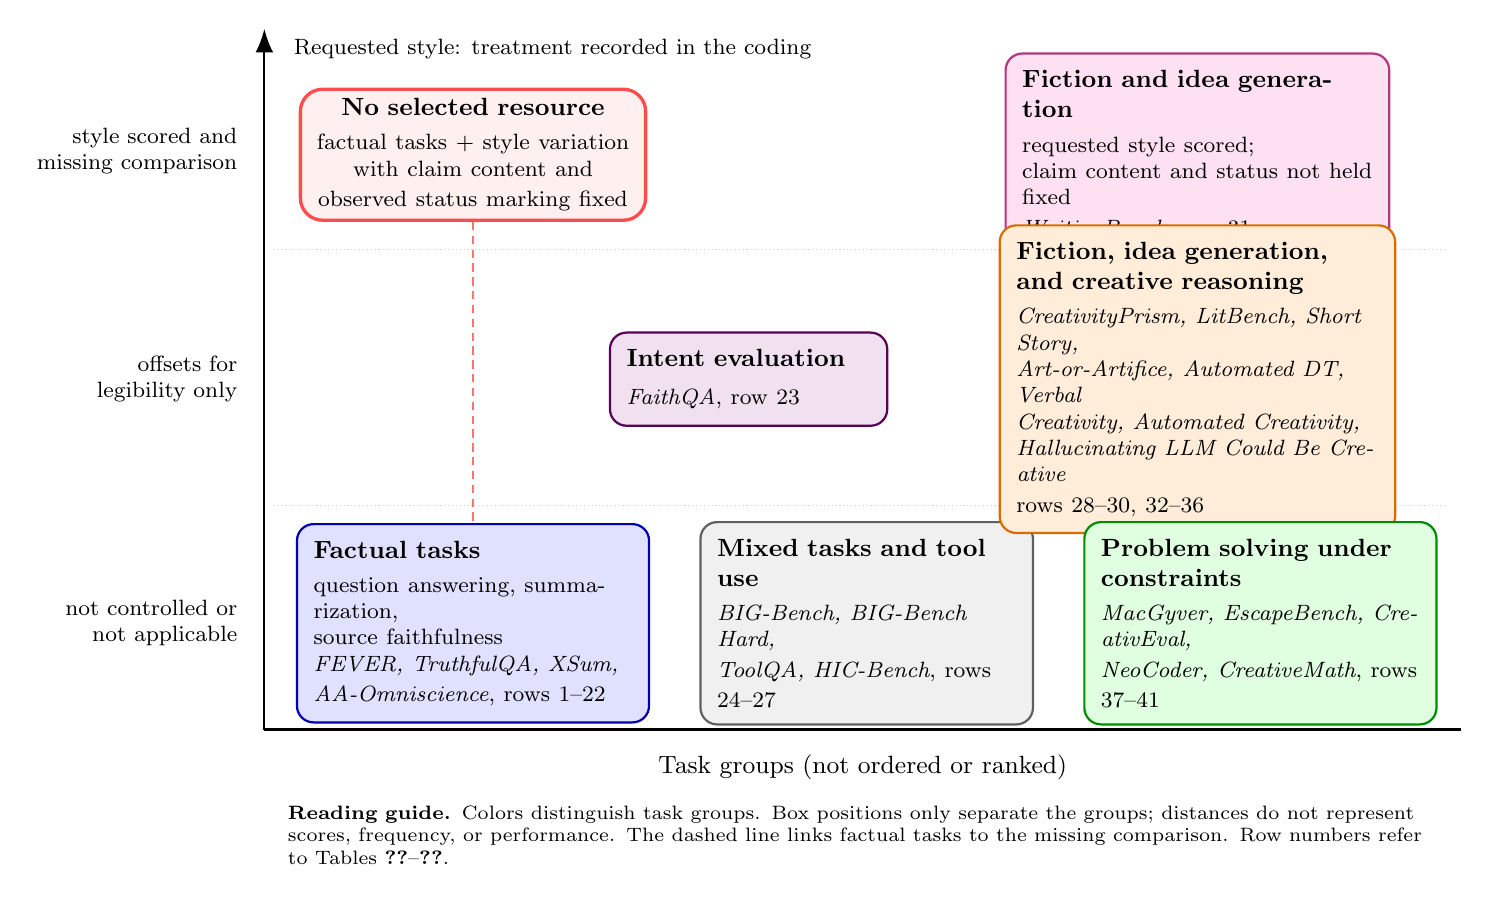
\begin{tikzpicture}[
    x=1cm,y=1cm,>=Latex,font=\small,
    axis/.style={thick,-{Latex[length=3mm]}},
    clusterbox/.style={
        rounded corners=6pt,thick,align=left,inner sep=6pt,
        text width=3.9cm
    },
    note/.style={font=\scriptsize,align=left}
]
% Positions separate categorical groups; they do not encode measurements.
\draw[thick] (0,0) -- (15.2,0);
\node[below,align=center] at (7.6,-0.20)
    {Task groups (not ordered or ranked)};
\draw[axis] (0,0) -- (0,8.9);
\node[anchor=west,font=\footnotesize] at (0.25,8.65)
    {Requested style: treatment recorded in the coding};
\node[left,align=right,font=\footnotesize] at (-0.22,1.35)
    {not controlled or\\not applicable};
\node[left,align=right,font=\footnotesize] at (-0.22,4.45)
    {offsets for\\legibility only};
\node[left,align=right,font=\footnotesize] at (-0.22,7.35)
    {style scored and\\missing comparison};
\draw[densely dotted,gray!35] (0.12,2.85) -- (15.0,2.85);
\draw[densely dotted,gray!35] (0.12,6.10) -- (15.0,6.10);

\node[
    draw=red!70,very thick,rounded corners=8pt,fill=red!6,
    text width=4.15cm,minimum height=1.65cm,align=center
] (gap) at (2.65,7.30) {
    \textbf{No selected resource}\\[1mm]
    \footnotesize factual tasks + style variation\\
    \footnotesize with claim content and\\
    \footnotesize observed status marking fixed
};

\node[clusterbox,draw=magenta!70!black,fill=magenta!12,
    text width=4.45cm] (writing) at (11.85,7.30) {
    {\bfseries Fiction and idea generation}\\[1mm]
    \footnotesize requested style scored;\\
    \footnotesize claim content and status not held fixed\\
    \footnotesize \textit{WritingBench}, row 31
};

\node[clusterbox,draw=blue!70!black,fill=blue!12,
    text width=4.05cm] (strict) at (2.65,1.35) {
    {\bfseries Factual tasks}\\[1mm]
    \footnotesize question answering, summarization,\\
    \footnotesize source faithfulness\\
    \footnotesize \textit{FEVER, TruthfulQA, XSum,}\\
    \footnotesize \textit{AA-Omniscience}, rows 1--22
};

\node[clusterbox,draw=violet!70!black,fill=violet!12,
    text width=3.10cm] (intent) at (6.15,4.45) {
    {\bfseries Intent evaluation}\\[1mm]
    \footnotesize \textit{FaithQA}, row 23
};

\node[clusterbox,draw=gray!75!black,fill=gray!12,
    text width=3.80cm] (mixed) at (7.65,1.35) {
    {\bfseries Mixed tasks and tool use}\\[1mm]
    \footnotesize \textit{BIG-Bench, BIG-Bench Hard,}\\
    \footnotesize \textit{ToolQA, HIC-Bench}, rows 24--27
};

\node[clusterbox,draw=orange!85!black,fill=orange!15,
    text width=4.60cm] (creative) at (11.85,4.45) {
    {\bfseries Fiction, idea generation,}\\
    {\bfseries and creative reasoning}\\[1mm]
    \footnotesize \textit{CreativityPrism, LitBench, Short Story,}\\
    \footnotesize \textit{Art-or-Artifice, Automated DT, Verbal}\\
    \footnotesize \textit{Creativity, Automated Creativity,}\\
    \footnotesize \textit{Hallucinating LLM Could Be Creative}\\
    \footnotesize rows 28--30, 32--36
};

\node[clusterbox,draw=green!55!black,fill=green!12,
    text width=4.05cm] (solution) at (12.65,1.35) {
    {\bfseries Problem solving under constraints}\\[1mm]
    \footnotesize \textit{MacGyver, EscapeBench, CreativEval,}\\
    \footnotesize \textit{NeoCoder, CreativeMath}, rows 37--41
};

\draw[densely dashed,red!55,line width=0.7pt]
    (gap.south) -- (gap.south |- strict.north);
\node[note,text width=14.6cm,anchor=north] at (7.6,-0.85) {
    \textbf{Reading guide.}
    Colors distinguish task groups. Box positions only separate the groups;
    distances do not represent scores, frequency, or performance.
    The dashed line links factual tasks to the missing comparison.
    Row numbers refer to
    Tables~\ref{tab:full-mapping-factual-a}--\ref{tab:full-mapping-creative}.
};
\end{tikzpicture}%
}
\caption{\textbf{Task groups and requested style in the selected resources.}
WritingBench is the only entry coded as scoring requested style, but it does
not hold claim content and observed status marking fixed. No entry records
a style comparison that keeps both fixed. The red box highlights this
missing comparison for factual tasks; it is not an additional resource.
The figure summarizes the current coding in Appendix~\ref{app:mapping},
which still needs independent verification. It does not measure evaluator
performance or display the other truth-contract fields.}
\label{fig:profiles}
\end{figure}
\FloatBarrier

\section{Exemples}\label{sec:cases}

We present five cases to illustrate how the rule applies when a reference, instruction,
claim, or response wording changes. These examples explain the rule; they are not
model outputs collected in an experiment. Each states what stays the same, what changes,
and which label the rule predicts. Case~B changes several conditions together.
Case~E can test an evaluator only after an independent check confirms that
the versions express the same claim with the same status.
Figure~\ref{fig:case-transitions} provides a compact guide.

\begin{figure}[!ht]
\centering
\resizebox{\textwidth}{!}{%
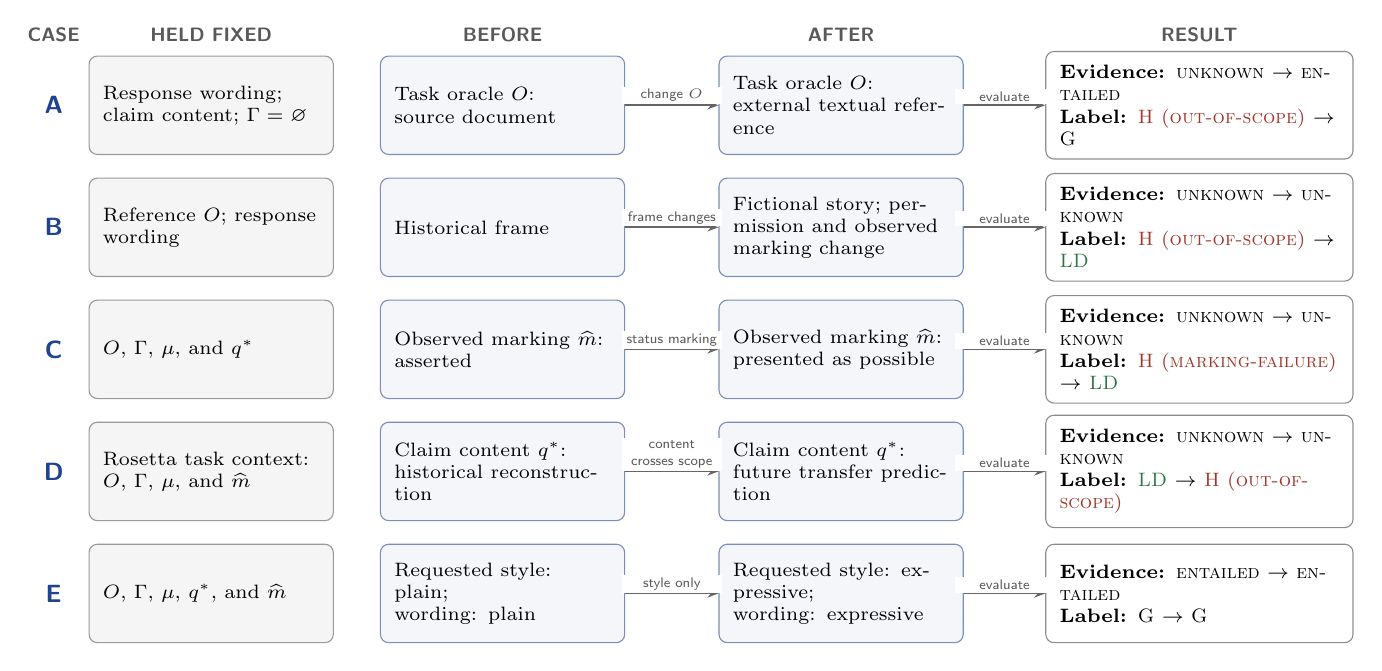
\begin{tikzpicture}[x=1cm,y=1cm,font=\small,
  every node/.style={inner sep=0pt}]
  \definecolor{caseblue}{RGB}{31,67,140}
  \definecolor{casegreen}{RGB}{42,118,67}
  \definecolor{casered}{RGB}{162,54,42}
  \tikzset{
    colhead/.style={font=\scriptsize\sffamily\bfseries,text=black!65,
      align=center},
    caselabel/.style={font=\small\sffamily\bfseries,text=caseblue,
      align=center},
    fixed/.style={rectangle,rounded corners=3pt,draw=black!40,fill=gray!8,
      text width=2.75cm,minimum height=1.25cm,align=left,
      font=\scriptsize,inner sep=5pt},
    condition/.style={rectangle,rounded corners=3pt,draw=caseblue!60,
      fill=caseblue!5,text width=2.75cm,minimum height=1.25cm,
      align=left,font=\scriptsize,inner sep=5pt},
    outcome/.style={rectangle,rounded corners=3pt,draw=black!45,fill=white,
      text width=3.55cm,minimum height=1.25cm,align=left,
      font=\scriptsize,inner sep=5pt},
    transition/.style={-{Stealth[length=4pt,width=3pt]},semithick,
      draw=black!60},
    transitionlabel/.style={font=\tiny\sffamily,text=black!65,
      align=center,text width=1.20cm,fill=white,inner sep=1pt},
    beforeafter/.style={font=\tiny\sffamily\bfseries,text=black!55,
      align=center}
  }

  \node[colhead] at (0,0.90) {CASE};
  \node[colhead] at (2.00,0.90) {HELD FIXED};
  \node[colhead] at (5.70,0.90) {BEFORE};
  \node[colhead] at (10.00,0.90) {AFTER};
  \node[colhead] at (14.55,0.90) {RESULT};

  % Case A
  \node[caselabel] at (0,0) {A};
  \node[fixed] (a-fixed) at (2.00,0)
    {Response wording; claim content; $\Gamma=\varnothing$};
  \node[condition] (a-before) at (5.70,0)
    {Task oracle $O$:\\source document};
  \node[condition] (a-after) at (10.00,0)
    {Task oracle $O$:\\external textual reference};
  \draw[transition] (a-before.east) --
    node[transitionlabel,above] {change $O$} (a-after.west);
  \node[outcome] (a-result) at (14.55,0)
    {\textbf{Evidence:} \textsc{unknown} $\to$ \textsc{entailed}\\
     \textbf{Label:} \textcolor{casered}{\Hall{} (\textsc{out-of-scope})}
     $\to$ \Grd};
  \draw[transition] (a-after.east) --
    node[transitionlabel,above] {evaluate} (a-result.west);

  % Case B
  \node[caselabel] at (0,-1.55) {B};
  \node[fixed] (b-fixed) at (2.00,-1.55)
    {Reference $O$; response wording};
  \node[condition] (b-before) at (5.70,-1.55)
    {Historical frame};
  \node[condition] (b-after) at (10.00,-1.55)
    {Fictional story; permission and observed marking change};
  \draw[transition] (b-before.east) --
    node[transitionlabel,above] {frame changes} (b-after.west);
  \node[outcome] (b-result) at (14.55,-1.55)
    {\textbf{Evidence:} \textsc{unknown} $\to$ \textsc{unknown}\\
     \textbf{Label:} \textcolor{casered}{\Hall{} (\textsc{out-of-scope})}
     $\to$ \textcolor{casegreen}{\LD}};
  \draw[transition] (b-after.east) --
    node[transitionlabel,above] {evaluate} (b-result.west);

  % Case C
  \node[caselabel] at (0,-3.10) {C};
  \node[fixed] (c-fixed) at (2.00,-3.10)
    {$O$, $\Gamma$, $\mu$, and $q^*$};
  \node[condition] (c-before) at (5.70,-3.10)
    {Observed marking $\widehat{m}$:\\asserted};
  \node[condition] (c-after) at (10.00,-3.10)
    {Observed marking $\widehat{m}$:\\presented as possible};
  \draw[transition] (c-before.east) --
    node[transitionlabel,above] {status marking} (c-after.west);
  \node[outcome] (c-result) at (14.55,-3.10)
    {\textbf{Evidence:} \textsc{unknown} $\to$ \textsc{unknown}\\
     \textbf{Label:} \textcolor{casered}{\Hall{} (\textsc{marking-failure})}
     $\to$ \textcolor{casegreen}{\LD}};
  \draw[transition] (c-after.east) --
    node[transitionlabel,above] {evaluate} (c-result.west);

  % Case D
  \node[caselabel] at (0,-4.65) {D};
  \node[fixed] (d-fixed) at (2.00,-4.65)
    {Rosetta task context:\\$O$, $\Gamma$, $\mu$, and $\widehat{m}$};
  \node[condition] (d-before) at (5.70,-4.65)
    {Claim content $q^*$:\\historical reconstruction};
  \node[condition] (d-after) at (10.00,-4.65)
    {Claim content $q^*$:\\future transfer prediction};
  \draw[transition] (d-before.east) --
    node[transitionlabel,above] {content crosses scope} (d-after.west);
  \node[outcome] (d-result) at (14.55,-4.65)
    {\textbf{Evidence:} \textsc{unknown} $\to$ \textsc{unknown}\\
     \textbf{Label:} \textcolor{casegreen}{\LD} $\to$
     \textcolor{casered}{\Hall{} (\textsc{out-of-scope})}};
  \draw[transition] (d-after.east) --
    node[transitionlabel,above] {evaluate} (d-result.west);

  % Case E
  \node[caselabel] at (0,-6.20) {E};
  \node[fixed] (e-fixed) at (2.00,-6.20)
    {$O$, $\Gamma$, $\mu$, $q^*$, and $\widehat{m}$};
  \node[condition] (e-before) at (5.70,-6.20)
    {Requested style: plain;\\wording: plain};
  \node[condition] (e-after) at (10.00,-6.20)
    {Requested style: expressive;\\wording: expressive};
  \draw[transition] (e-before.east) --
    node[transitionlabel,above] {style only} (e-after.west);
  \node[outcome] (e-result) at (14.55,-6.20)
    {\textbf{Evidence:} \textsc{entailed} $\to$ \textsc{entailed}\\
     \textbf{Label:} \Grd{} $\to$ \Grd{}};
  \draw[transition] (e-after.east) --
    node[transitionlabel,above] {evaluate} (e-result.west);
\end{tikzpicture}%
}
\caption{\textbf{Five examples as a transition diagram.}
Each row shows what stays fixed, what changes, and the expected evidence
state and label. Case~B changes several conditions together. Case~E changes
both the requested style and the response's wording. These are expected
results from the rule, not results measured on model outputs.}
\label{fig:case-transitions}
\end{figure}
\FloatBarrier
\paragraph{Case A: changing the task oracle}
In XSum \citep{maynez_faithfulness_2020}, a text summarization dataset, a summary statement may be absent from the source document while
remaining correct against external evidence .
Consider a claim that the source document neither supports nor contradicts,
but that a specified external reference supports.
\textbf{Purpose.} To illustrate why the oracle used for evaluation matters.
\par\textbf{Fixed.} The response wording, claim content, and permission scope
$\Gamma=\varnothing$, which allows only supported content.
\par\textbf{Changed.} One condition uses the source document as the task oracle;
the other design uses a fixed collection of external textual evidence.
Each reference remains fixed within its own design.
\par\textbf{Predicted result.} Relative to the source document, the claim is
\textsc{unknown}. Because $\Gamma=\varnothing$, it receives the hallucination
label with reason code \textsc{out-of-scope}. Relative to the external task
oracle, the same claim is \textsc{entailed}  and receives the  label $\Grd$
.

\paragraph{Case B: moving from a factual context to a fictional story}
This case changes both what the task permits and how the response presents
the content. It does not isolate permission alone.
\textbf{Purpose.} To distinguish a claim presented as historical fact from
the same placement proposed as part of a fictional story.
\par\textbf{Fixed.} The Rosetta Stone reference and the example sentence
string ``The complete stele stood near a temple entrance.''
\par\textbf{Changed.} The historical condition asks for a museum label using
only supported information. The fictional condition permits an invented setting and places
the same sentence inside a declared alternate-history story. Permission and
observed status marking change; the reference does not.
\par\textbf{Predicted result.} Here, the content checked against the historical
reference is the proposed temple-entrance placement; its fictional status is
recorded in the observed marking. The reference neither supports nor
contradicts that placement, so its evidence state remains \textsc{unknown}.
In the historical condition, $\Gamma=\varnothing$, so
it receives the hallucination label with reason code \textsc{out-of-scope}.
In the fictional condition, the task permits the placement and the declared
frame supplies the required marking, so it receives licensed divergence.
This treatment applies to the placement proposed within the story. A response
reporting what a story says would express a different claim and would need
to be checked as such. Identical wording alone does not guarantee identical
claim content.

\paragraph{Case C: changing the observed status marking}
This comparison reuses the Rosetta Stone reconstruction from
Section~\ref{subsec:contract}. The permission scope allows a plausible
placement, and the required status marking requires presenting it as a
possibility. The request for one reconstruction is a separate limit on the
whole response.
\textbf{Purpose.} To illustrate that permission alone is not enough: presentation is
part of the contract.
\par\textbf{Fixed.} The task oracle $O$, $\Gamma$, $\mu$, the content $q^*$
that the complete stele stood near a temple entrance, and its \textsc{unknown}
evidence state.
\par\textbf{Changed.} Only the observed status marking $\widehat{m}$.
\par\textbf{Predicted result.} ``The complete stele stood near a temple
entrance'' receives the hallucination label with reason code
\textsc{marking-failure}. ``One possible reconstruction places the complete
stele near a temple entrance'' receives the licensed-divergence label. The
content, evidence state, and all three contract fields are identical; only the
wording that presents the placement as established or possible differs.

\paragraph{Case D: testing a scope boundary}
This case returns to the Rosetta Stone task. Permission covers a plausible
historical reconstruction, and required marking identifies it as a possibility.
\textbf{Purpose.} To show that presenting content as possible does not make
it permitted: its topic must also fall within the scope.
\par\textbf{Fixed.} The task oracle $O$, $\Gamma$, $\mu$, the \textsc{unknown}
evidence state, and observed marking $\widehat{m}$ presenting the content as possible.
\par\textbf{Changed.} Only the content $q^*$: ``One possible reconstruction
places the complete stele near a temple entrance'' versus the constructed
prediction ``One possibility is that the stone will be returned to Egypt next
year.''
\par\textbf{Predicted result.} The historical reconstruction lies inside
$\Gamma$ and receives the licensed-divergence label. The future transfer
prediction is also \textsc{unknown} and marked as a possibility, but it is not
the historical reconstruction that the task permits. It falls outside
$\Gamma$ and receives the hallucination label with reason code
\textsc{out-of-scope}.

\paragraph{Case E: changing the wording while preserving the claim}
This case compares two styles that express the same content as established
fact.
\textbf{Purpose.} To illustrate the label that should remain unchanged when
wording changes but content and status do not.
\par\textbf{Fixed.} The task oracle $O$ of the Rosetta Stone example of
Figure~\ref{fig:claim-label-annotation}, $\Gamma$, $\mu$, the content component
$q^*$ that the decree on the Rosetta stone appears in hieroglyphic, Demotic, and Greek, and the
observed status marking $\widehat{m}$.
\par\textbf{Changed.} The requested style and the response's wording change
together. Both versions are intended to preserve the claim content and status.
Plain wording: ``The decree is written in hieroglyphic, Demotic, and
Greek.''
Expressive wording: ``The same message speaks three times over: once in
hieroglyphs, once in Demotic, once in Greek.''
\par\textbf{Predicted result.} An evaluator should recover the same claim
from both versions and assign the grounded label, since the oracle supports
it. Whether each version uses the requested style is assessed separately.
After an independent check confirms equal content and status, a difference
in recovered claims or labels would indicate an evaluator error on this test.
One such result would not establish how often style affects claim recovery.

These cases give expected labels under stated conditions. The next step is
to test whether evaluators identify those conditions reliably and produce
the expected labels. The research agenda sets out those studies.


\section{Research Agenda}\label{sec:agenda}

The agenda contains three main questions: can evaluators apply the framework reliably,
does stating the contract explicitly help evaluation, and does the approach
work in other settings? Table~\ref{tab:agenda} groups seven priorities around
these questions. Priorities 1--3 concern reliable annotation and checking;
Priorities 4--5 concern practical use; Priorities 6--7 concern other domains
and tasks that change over time.

Studies should compare the framework with a method that already checks both
factuality and task instructions. To test the labeling rule, both methods
should use the same oracle and recovered claims. To test claim recovery,
the study should instead vary that step explicitly. Independent annotators
should record evidence, permission, marking, and whether the response is
acceptable for the task. If all reference judgments simply follow our rule,
agreement only shows that a method applies it correctly; it does not show
that the rule is useful or acceptable. The comparison criteria and thresholds
should be fixed before evaluation.

\begin{table}[!ht]
\centering
\small
\setlength{\tabcolsep}{5pt}
\renewcommand{\arraystretch}{1.10}
\caption{\textbf{The research agenda in one view.} The table lists seven
priorities and their open questions. The corresponding paragraphs give the
study designs, measures, and critical comparisons.}
\label{tab:agenda}
\begin{tabularx}{\linewidth}{@{}P{0.24\linewidth}Y@{}}
\toprule
\textbf{Priority} & \textbf{Open question}\\
\midrule
1.~Contract annotation
& Can evaluators consistently identify the task oracle $O$, permission scope
$\Gamma$, and required status marking $\mu$ from a task context?\\\addlinespace[2pt]
2.~Controlled comparisons
& Do claim labels change as predicted when one contract field changes and the rest are held fixed?\\\addlinespace[2pt]
3.~Recovery across styles
& Does the evaluator recover the same content and status when only wording changes?\\\addlinespace[2pt]
4.~Response-level record
& What must be added to a claim trace to judge a complete response?\\\addlinespace[2pt]
5.~Reducing hallucination
& Can hallucination be reduced while keeping useful content that the task permits?\\\addlinespace[2pt]
6.~Generalization
& Do the contract fields remain applicable across other domains, genres, and
languages?\\\addlinespace[2pt]
7.~Changing tasks and actions
& When should a contract be updated, and how can an incorrect claim affect a later action?\\
\bottomrule
\end{tabularx}
\end{table}
\FloatBarrier

\paragraph{1. Contract annotation}
A public annotation guide should explain which sources and checks the oracle
uses, what content is permitted, how it must be presented, and how claims are
interpreted. Pilot studies should annotate each field separately. They should
measure initial agreement, how often disagreements require a further decision,
annotation time, and the causes of errors. Contract annotations can be reused
for the same task, but claims must be recovered from each response.
\emph{Critical test.} If annotators repeatedly disagree about a field, its
definition may not be precise enough to apply reliably. If annotation takes
more time without helping explain errors, its practical benefit is limited.

\paragraph{2. Controlled comparisons}
A benchmark should compare tasks that differ in permission scope or required
marking while keeping the oracle fixed. Comparisons of different oracles
require separate evaluation designs, each with its own fixed reference.
For example, compare the same contradicted claim under tasks that permit
or forbid that change. The protocol must distinguish changing what marking
is required ($\mu$) from changing what the response actually shows
($\widehat{m}$), as Case~C does. A change from historical to fictional framing,
as in Case~B, may also change the claim's meaning and requires separate analysis.

Studies should record evidence states, labels, reason codes, and independent
judgments of whether the content meets the task's requirements. They should
also examine whether annotators accept the proposed labels for permitted
contradictions and for supported facts explicitly excluded by a requirement
for invention.
\emph{Critical test.} A comparison does not isolate one condition if it also
changes the claim's meaning. If independent judgments consistently reject
the proposed labels in those cases, the convention needs reconsideration.
If a comparison method using the same information is equally accurate and
informative, a separate implementation has no demonstrated advantage there.

\paragraph{3. Claim recovery across styles}\label{par:style-scale}
As a provisional style scale, we distinguish minimally marked, locally
marked, and sustained marked style, indexed by $\sigma\in\{0,1,2\}$ when
needed. These levels describe how much the wording differs from plain prose,
not a particular named style, creativity, or factuality. Their boundaries
require empirical validation.

The study should compare different wordings of the same claim content and
status under the same contract. An independent check must confirm that
$q^*$ and $\widehat{m}$ remain the same. The evaluation should record missed
or added claims, claims incorrectly merged or split, changes in recovered
status, and resulting label errors.

A separate comparison can give an evaluator access to the requested style
or withhold that information while keeping the response fixed. This tests
whether the request helps interpret the response. In both studies, the trace
should show whether an error arose while recovering the claim, checking
evidence, or applying the contract.
\emph{Critical test.} Different results for versions independently confirmed
to express the same content and status show a robustness problem. The trace
is useful only if it helps identify where such errors occur.

\paragraph{4. Response-level evaluation}
To measure recovery coverage, evaluators need an independently checked list
of the claims expressed in the response. They compare the recovered claims
with that list, preserving their meaning. This measures how much of the
response was recovered, not whether it supplied everything the task requested.
Possible summaries include counts of each label, a flag for any hallucination,
or a score that gives more weight to serious errors. Studies must test how
useful these summaries are and how missed claims affect them.

Studies should compare these overall judgments with independent assessments of
reasoning, consistency, completeness, relevance, and task success. They should
also examine how many claims must be recovered and how to check limits such
as the requested number of reconstructions. Comparing several ways to combine
labels shows whether conclusions or model rankings depend on that choice.
Style and creativity remain separate reported outcomes.
\emph{Critical test.} An additional check has limited practical value in a
setting if it provides no information beyond the trace. This does not mean
that claim labels guarantee the correctness of the whole response.

\paragraph{5. Reducing hallucination while keeping permitted content}
A method may reduce hallucination simply by producing less content,
including hypotheses that the task requested or allowed. Studies should
compare retrieval, verification, abstention, and generation constrained by
rules on both error reduction and preservation of useful content. Report
grounded and licensed content, style, and creative-task success separately
for each contract. Report uncertainty in human creativity judgments and
show these different outcomes rather than hiding them in one overall score.
\emph{Critical test.} A method that improves only by removing permitted
content has not established a benefit for tasks requiring such content.

\paragraph{6. Generalization}
Repeat the annotation studies and controlled comparisons in other domains,
genres, and languages. Report agreement and cost for each field separately:
identifying permission and interpreting uncertainty can cause different
difficulties. The provisional style scale also needs testing beyond the
museum examples.
\emph{Critical test.} Repeated disagreement in a particular domain or
language limits where the relevant definition or procedure can be applied.

\paragraph{7. Updating contracts during tasks and actions}
In a task with several steps, new evidence may become available and later
actions may rely on earlier claims. Extending the framework would require
recording the contract used at each step. Studies should explain why the
oracle or permission changed and follow how an incorrect claim affects later
actions. Updates must follow the task protocol; they cannot be made afterward
to excuse a response.
\emph{Critical test.} If an evaluation using one fixed contract performs
equally well on the chosen action outcomes, the extension has no measured
benefit in that setting.

\section{Discussion}\label{sec:discussion}

\subsection{What Is Relative and What Is Not}\label{subsec:relative}

Our position concerns the conditions for assigning an evaluation label.
A task can authorize a possibility without making it true. Likewise,
changing the designated oracle changes the evidence relation used for
evaluation, not the underlying world's facts. Under the proposed convention,
H covers unknown or contradicted content that is not permitted or not presented
as required. It also covers supported facts explicitly excluded by a requirement
for invented content. A permitted contradiction remains contradicted even when
it receives LD, just as an excluded supported fact remains entailed when it
receives H. Studies must test whether annotators understand and accept these
uses of the labels. Keeping the evidence state and reason code makes the
different cases visible even when the label itself is disputed.

Theoretical work provides context for reliability concerns. Some results
describe minimum error rates under assumptions about how a model expresses
confidence; others examine what a computational system can guarantee
\citep{kalai_calibrated_2024,xu_hallucination_2024,banerjee_llms_2024}.
Their assumptions differ, and they do not fix the error rate of every
deployed model or rule out negligible rates in a specific setting
\citep{suzuki_negligible_2025}. Our argument does not require proving that
hallucination is unavoidable: it concerns how to evaluate content against
specified evidence and task conditions.

The AA-Omniscience snapshot provides a descriptive
illustration \citep{jackson_aaomniscience_2025,artificialanalysis_omniscience_leaderboard_2026}.
Appendix~\ref{app:omniscience} gives its date, metrics, and limitations.
Comparing different models at one time does not isolate the effect of model
size or show that truth-contract annotation improves evaluation.

\subsection{Interpreting the Response-Level Record}

Section~\ref{subsec:response} leaves open how claim labels should be combined.
A favorable overall judgment would apply only to the claims actually checked
and the declared requirements for coverage. It would not guarantee that the
response is factual, creative, or complete. The optional rule in
Appendix~\ref{app:diagnostics} uses \textsc{indeterminate} when the evaluation
cannot be completed. This records a limit of the evaluation, not necessarily
an error by the model, and should be reported.

These distinctions matter for mitigation. A claim trace can reveal whether a
method reduced contradictions, removed unauthorized additions, or improved
marking. Creative-task assessment then asks whether useful permitted content
was preserved. Giving more weight to serious errors may help decide which
responses to review first. That score cannot change the labels of their
individual claims.

\subsection{Limitations and Open Decisions}

The framework proposes rules for evaluating claims; it has not yet been
validated as an evaluator. Applying it requires claims that can be interpreted
reliably, a specified contract, and dependable evidence checks. Separating
content ($q^*$) from observed marking ($\widehat{m}$) is difficult when words
such as ``may'' or a fictional setting change the meaning. Unresolved cases
must be recorded as evaluation failures.

Claim labels also leave questions about the whole response unanswered. They
do not establish that its reasoning is valid, its claims are mutually
consistent, or it supplies all requested information. They do not enforce
limits such as the number of reconstructions requested. Those checks need
their own rules and validation, as discussed in Priority~4.


\section{Conclusion}\label{sec:conclusion}

We argue that hallucination evaluation needs an explicit truth contract.
The evidence check establishes whether a claim is supported, contradicted,
or unknown. The task specifies what content is permitted or excluded and how
it must be presented. Keeping these questions separate makes the reason for
each claim label explicit, while creativity and overall task success remain
separate assessments.

The proposed rule, descriptive comparison, and examples provide a
basis for testing this approach. The next step is to determine whether
evaluators can apply it reliably and whether it helps compared with methods
using the same evidence and instructions. These studies should test both
whether facts are checked correctly and whether permitted additions are
recognized and presented as required.
\clearpage

\appendix

\appendixsection{Response-Level Record, Procedural Failures, and Optional Aggregation}%
\phantomsection
\makeatletter\def\@currentlabel{A}\makeatother\label{app:diagnostics}

Section~\ref{sec:framework} defines how to recover, verify, and label claims.
This appendix explains what to report: the individual decisions, any
evaluation failures, and separate assessments of style and creativity.
It also describes an optional way to combine labels and a formal test of
claim recovery across styles.


\paragraph{Reporting and aggregation details}
Section~\ref{subsec:response} defines the claim trace and leaves the global
verdict as a research question. One possible rule requires a minimum level
of recovery coverage, declared before evaluation, and follows this order:
\begin{enumerate}
\item Report \textsc{contract-violating} if any reliably checked claim receives H.
\item Otherwise, report \textsc{indeterminate} if too few claims were recovered
or a failure prevents the required checks.
\item Otherwise, report \textsc{contract-compliant} for the completed checks.
\end{enumerate}
This is an option to test, not the framework's default. A study using it must
publish its coverage threshold, claim trace, and evaluation failures. A
favorable result cannot certify claims that were not recovered.

Style-marking alignment is \textsc{match}, \textsc{mismatch}, or
\textsc{not applicable} when the task specifies no target. Compare the requested
level with the independently assessed observed level using the provisional
three-level scale in Priority~3 of Section~\ref{sec:agenda}
(page~\pageref{par:style-scale}). If either level cannot be determined,
report that the comparison could not be completed, rather than a mismatch.
A future validated rule could allow a small difference between levels
instead of requiring an exact match.

Creative-task success is \textsc{pass}, \textsc{fail}, \textsc{not assessed},
or a task-specific score under stated criteria. Report those criteria and
unit of analysis. Novelty, usefulness, quality, and diversity should not be
silently substituted for one another.

An overall score may use label proportions, give more weight to serious
errors, or follow task-specific rules. State the rule before evaluation,
retain every claim label, and report whether other reasonable rules change
the conclusions. Checks of reasoning, consistency, completeness, relevance,
and the number of requested additions remain separate.

Claims that are individually permitted may contradict one another. If the
oracle is consistent and claims are correctly interpreted in the same context,
however, two contradictory claims cannot both be entailed. An apparent case
requires checking the oracle and recovered claims before interpreting the labels.

\paragraph{Procedural failures}

A \emph{procedural failure} occurs when the evaluator cannot complete a
required step. It is recorded instead of assigning \Grd, \Hall, or \LD{} to
the affected content. Labeling requires a claim with a clear meaning, a
specified contract, and a completed evidence check. The protocol specifies
the oracle; the task conditions specify permission and required marking.
The following failures prevent one or more of these requirements from being met.

\paragraph{Failures of claim recovery}
The evaluator may miss a claim, add one absent from the response, merge claims
that need separate checks, or split one claim into redundant parts. It may
also change the meaning or observed status while recovering a claim.
Here, \emph{canonicalization} means expressing the recovered content as
$q^*$ while preserving its meaning and context. It is part of claim recovery,
not an additional stage of the oracle. If the meaning of the affected text
cannot be resolved, no label is assigned to it.

\paragraph{Failures of the truth contract or task oracle}
The evaluator may instead be unable to apply the contract to a claim it has
recovered. Four failures have this effect.
\begin{description}
  \item[Truth-contract specification failure.] The protocol and task conditions
        do not specify which oracle to use, what content is permitted or
        excluded, or how it must be presented.
  \item[Task-oracle specification failure.] The oracle's sources or checks are
        not defined precisely enough. For text, this can include unclear source
        authority, dates of validity, or rules for resolving conflicting evidence.
  \item[Task-oracle adequacy failure.] Required sources or checks are unavailable,
        a source version does not meet the protocol, or an unresolved conflict
        prevents the specified procedure from being applied.
  \item[Adjudication failure.] The evaluator cannot reach one evidence state
        using the specified procedure.
\end{description}
In each case the evaluator records the failure and leaves the affected span
unlabeled.
An available source that neither supports nor contradicts a claim can yield
\textsc{unknown} after a completed check. A source that cannot be accessed
instead prevents that check. The failure must not be automatically converted
to \textsc{unknown}. Under the optional overall reporting rule above, a
reliably checked H takes priority; otherwise a blocking failure produces
\textsc{indeterminate}.

Recent fact-verification work examines difficulties in separating such
outcomes. The way unknown examples are built affects what a verifier learns
and may hide difficulty in deciding the evidence state
\citep{qiu_evidence_2026}. Separately, a single global faithfulness label can
hide disagreement about individual sentences through an averaging bias
\citep{zhang_averaging_2026}.

\paragraph{An example}
Suppose two annotators read the closing span of a museum panel, ``the winter
that would not lift''.
One recovers a claim about the severity of that winter; the other recovers no
truth-conditional claim at all.
The two annotators disagree about which claim the span commits to, not about
which label a shared claim deserves.
The evaluators must first try to resolve the difference in interpretation.
If it remains unresolved, they record a claim-recovery failure for that text,
rather than compare labels assigned to different interpretations.

A response that does not use the requested style is not a
procedural failure.
That mismatch is recorded separately, while a recovered claim that violates
the truth contract receives its claim label.


\paragraph{Claim-preserving style variation test}
The test uses three responses whose content and status have been independently
checked as equivalent, but whose wording differs in style. It asks whether
the evaluator recovers the same claims and assigns the same labels.

Let $y_0,y_1,y_2$ denote the responses and $p_0,p_1,p_2$ their task contexts.
The contexts differ only in the requested style level:
$\sigma_{p_0}=0$, $\sigma_{p_1}=1$, and $\sigma_{p_2}=2$, using the provisional
scale from Priority~3. Each recovered claim is represented by its content
and observed marking, $c^*=(q^*,\widehat{m})$. After independently matching
the claims one to one, let $\mathcal C^*(y_i,p_i)$ denote their set for each
response. Equal content and status across versions require
$\mathcal C^*(y_0,p_0)=\mathcal C^*(y_1,p_1)=\mathcal C^*(y_2,p_2)$.
Thus, matched claims retain the same $q^*$ and $\widehat{m}$ components, although their
wording and observed style levels may differ. With $O$,
$\Gamma$, and $\mu$ fixed, every matched canonical claim $c_j^*$ must also
receive the same claim label (\Grd, \Hall, or \LD) under $y_0,p_0$, $y_1,p_1$,
and $y_2,p_2$.

\begin{itemize}
  \item \emph{Claim recovery error}: a claim is missed or content absent
        from the response is added.
  \item \emph{Canonicalization error}: the recovered representation changes
        the claim's meaning or observed status.
  \item \emph{Claim-label instability}: matched canonical claims receive
        different labels when $O$, $\Gamma$, and $\mu$ are fixed.
  \item \emph{Style-marking alignment error}: the evaluator
        incorrectly classifies the match between requested and observed
        style-marking levels.
\end{itemize}

These error checks require independently verified matches between the
claims in the different versions. Checking style alignment also requires an
independent judgment of the requested and observed style levels.
Claim-label instability is an error only when $O$, $\Gamma$, and $\mu$ remain fixed.
When $\Gamma$ or $\mu$ changes, the same unsupported content may
intentionally change from the hallucination label to the licensed-divergence
label; its evidence state remains unchanged.

A separate question is whether changing the rule for combining labels changes
the ranking of responses. Such a change is not automatically an evaluator
error. Comparisons should report this sensitivity, while retaining the
individual labels and checks.

\appendixsection{Resource Mapping}%
\phantomsection
\makeatletter\def\@currentlabel{B}\makeatother\label{app:mapping}
\renewcommand*{\theHtable}{B.\arabic{table}}

Tables~\ref{tab:full-mapping-factual-a}--\ref{tab:full-mapping-creative} list
the forty-one selected resources. Each row records the oracle type and what
it uses, any separate quality or task-success criterion, treatment of the
requested style, permission scope $\Gamma$, and required status marking $\mu$.
Rows are grouped by task category, as summarized in Figure~\ref{fig:profiles}.

\paragraph{Coding vocabulary}
Each field uses one of the codes below. Text in parentheses gives details
about the task without adding another code. The labels are retained so the
tables can be checked; the current coding still requires independent
verification, including clearer criteria where categories overlap.

\begin{description}
  \item[Task category.]
  These categories describe types of tasks; %they do not rank them.
  The task types are: \emph{strict grounding};
  \emph{intent evaluation};
  \emph{declared-frame invention and ideation};
  \emph{constrained solution search};
  \emph{heterogeneous suites and tool use}.

  \item[Oracle reference or checking procedure (column $O$).]
  The codes include textual and nontextual checks. Each entry still needs
  verification that it checks the evaluated content rather than only overall
  task success.
  \emph{source document}, a supplied document treated as authoritative for
  evidence checking;
  \emph{retrieval set}, retrieved items used to verify claims;
  \emph{database or knowledge base}, a structured factual resource;
  \emph{gold labels}, reference answers or labels used for checking;
  \emph{environment or tool state}, observable state or tool output;
  \emph{human adjudication}, a specified procedure for human checking;
  \emph{fictional-world constraints}, established facts or rules within a
  specified fictional setting;
  \emph{mixed or task-dependent}, when the type varies across subtasks or
  combines types;
  \emph{none identifiable}, when our coding finds no standard that can
  establish or contradict the evaluated claims.
  This field records what is used to check content, not a general quality or
  task-success criterion.

  \item[Quality or task-success criterion.]
  \emph{not separately represented};
  \emph{quality or preference rubric};
  \emph{novelty or divergent-thinking rubric};
  \emph{feasibility or correctness criterion};
  \emph{specification or tests};
  \emph{mixed}.
  Here, \emph{not separately represented} means that no additional criterion
  is reported beyond agreement with the task oracle; ordinary accuracy against
  $O$ is not recoded as a separate task-success dimension.

  \item[Requested style.]
  \emph{not controlled} records no controlled comparison of requested style;
  \emph{not controlled or not applicable} also covers tasks to which the
  comparison may not apply;
  \emph{scored, not claim-controlled} records style scoring without keeping
  claim content and status fixed.

  \item[Permission scope $\Gamma$.]
  \emph{inferred empty} means that the coding infers that only supported
  content is allowed;
  \emph{implicit frame} means that permission is inferred from the task or
  fictional setting;
  \emph{partial} records only part of the permission conditions;
  \emph{task-specific} and \emph{subtask-specific} indicate that permission
  depends on the task or subtask;
  \emph{mixed} combines conditions;
  \emph{not separately represented} means that no separate permission field
  was identified.
  These descriptions explain the labels; they do not supply all the criteria
  needed to distinguish them reliably. The recorded coding criterion asks
  whether a specification, test, or instruction authorizes unknown content.
  It does not document a systematic check for permitted contradictions or
  explicit exclusions of supported facts. The protocols must be reexamined
  before this coding can be treated as covering the full definition of
  $\Gamma$ in Section~\ref{subsec:contract}.
  % AUTHOR ACTION: document the coding criteria and verify permission coverage
  % against the source protocols before changing any categories or counts.

  \item[Required status marking $\mu$.]
  \emph{not scored} means that required status marking is not evaluated as a
  separate dimension.
  \emph{not separated} means that a relevant required-status-marking criterion
  is included in a broader task evaluation rather than scored independently.
  The first description can overlap with the second. Reproducible coding
  requires a clearer criterion separating absence of a marking check from
  a check included in a broader score. The table retains the current labels;
  no resource has been reassigned here.
  % AUTHOR ACTION: verify the distinction against the protocols, then update
  % the definitions, assignments, and counts together if necessary.
\end{description}

The original resources do not necessarily use the term \emph{task oracle}.
These codes record our interpretation of the references and checks
available in each evaluation design; they do not imply that a source uses
truth-contract terminology.
A preference score, quality rubric, novelty score, general task-success
signal, LLM-judge preference, or nonfactual user instruction is not by itself
a task oracle.
It remains in the quality or task-success column unless the evaluation uses it
to establish or contradict a claim.

\begin{table*}[t]
\centering
\scriptsize
\setlength{\tabcolsep}{3pt}
\renewcommand{\arraystretch}{1.0}
\caption{\textbf{Factuality and faithfulness resources with the selected
purposive mapping values (part I).}
The recorded oracle reference or checking procedure is separate from quality
or task success. Textual and nontextual checks can serve as oracles when they
establish or contradict evaluated content. ``Not controlled'' does not mean
that a plain style is required.}
\label{tab:full-mapping-factual-a}
\begin{tabularx}{0.99\linewidth}{
  @{}P{0.17\textwidth}P{0.25\textwidth}
  P{0.15\textwidth}P{0.14\textwidth}Y@{}}
\toprule
\textbf{Resource}
& \textbf{Task and task oracle $O$}
& \textbf{Quality / success criterion}
& \textbf{Requested style}
& \textbf{$\Gamma$ permission scope /\newline $\mu$ status marking}\\
\midrule
\multicolumn{5}{l}{\textbf{Task category: strict grounding}}\\
1.~FEVER \citep{thorne_fever_2018} & Fact checking\newline $O$: source document (Wikipedia evidence sentences) & not separately represented & not controlled & $\Gamma$: inferred empty\newline $\mu$: not scored\\
2.~TruthfulQA \citep{lin_truthfulqa_2022} & Factual QA\newline $O$: mixed or task-dependent (sourced reference answers; human adjudication for generations) & quality or preference rubric (informativeness) & not controlled & $\Gamma$: inferred empty\newline $\mu$: not scored\\
3.~PopQA \citep{mallen_when_2023} & Long-tail QA\newline $O$: database or knowledge base (Wikidata) & not separately represented & not controlled & $\Gamma$: inferred empty\newline $\mu$: not scored\\
4.~SimpleQA \citep{wei_measuring_2024} & Factual QA\newline $O$: gold labels (verified reference answers) & not separately represented & not controlled & $\Gamma$: inferred empty\newline $\mu$: not scored\\
5.~TriviaQA \citep{joshi_triviaqa_2017} & Reading QA\newline $O$: mixed or task-dependent (gold answers plus Web/Wikipedia documents) & not separately represented & not controlled & $\Gamma$: inferred empty\newline $\mu$: not scored\\
6.~DefAn \citep{rahman_defan_2024} & Factual QA\newline $O$: gold labels (definitive reference answers) & mixed (prompt alignment and cross-run consistency) & not controlled & $\Gamma$: inferred empty\newline $\mu$: not scored\\
7.~HaluEval \citep{li_halueval_2023} & Multi-task hallucination recognition\newline $O$: mixed or task-dependent (task references or source text; Web-assisted adjudication) & mixed (specificity and relevance folded into some labels) & not controlled & $\Gamma$: inferred empty\newline $\mu$: not scored\\
8.~FactBench \citep{bayat_factbench_2024} & Open-ended factuality evaluation\newline $O$: retrieval set (Web-retrieved material) & not separately represented & not controlled & $\Gamma$: inferred empty\newline $\mu$: not scored\\
9.~HalluLens \citep{bang_hallulens_2025} & Extrinsic/intrinsic hallucination benchmark\newline $O$: mixed or task-dependent (Wikipedia, nonexistent entities, or task context) & mixed (correctness and refusal/acceptance) & not controlled & $\Gamma$: inferred empty\newline $\mu$: not separated\\
10.~FRANK \citep{pagnoni_understanding_2021} & Summarization\newline $O$: source document (source documents) & not separately represented & not controlled & $\Gamma$: inferred empty\newline $\mu$: not scored\\
11.~QAGS \citep{wang_asking_2020} & Summarization\newline $O$: source document (source documents) & not separately represented & not controlled & $\Gamma$: inferred empty\newline $\mu$: not scored\\
12.~SummEval \citep{fabbri_summeval_2021} & Summarization\newline $O$: source document (source documents) & mixed (automatic metrics and human summarization-quality judgments) & not controlled & $\Gamma$: inferred empty\newline $\mu$: not scored\\
13.~XSum \citep{narayan_xsum_2018} & Summarization\newline $O$: source document (BBC source article) & mixed (ROUGE, human preference, and information preservation) & not controlled & $\Gamma$: inferred empty\newline $\mu$: not scored\\
\bottomrule
\end{tabularx}
\end{table*}

\clearpage
\begin{table*}[t]
\centering
\scriptsize
\setlength{\tabcolsep}{3pt}
\renewcommand{\arraystretch}{1.0}
\caption{\textbf{Factuality, faithfulness, and adjacent resources in the
selected purposive mapping (part II).}
Rows 14--22 continue strict grounding, row 23 represents intent evaluation,
and rows 24--27 cover heterogeneous or task-dependent conditions.}
\label{tab:full-mapping-factual-b}
\begin{tabularx}{0.99\linewidth}{
  @{}P{0.17\textwidth}P{0.25\textwidth}
  P{0.15\textwidth}P{0.14\textwidth}Y@{}}
\toprule
\textbf{Resource}
& \textbf{Task and task oracle $O$}
& \textbf{Quality / success criterion}
& \textbf{Requested style}
& \textbf{$\Gamma$ permission scope /\newline $\mu$ status marking}\\
\midrule
\multicolumn{5}{l}{\textbf{Task category: strict grounding (continued)}}\\
14.~CNN/DailyMail \citep{hermann_teaching_2015,wang_asking_2020} & News corpus used in summarization evaluation\newline $O$: source document (news source article) & not separately represented & not controlled & $\Gamma$: inferred empty\newline $\mu$: not scored\\
15.~DelucionQA \citep{sadat_delucionqa_2023} & Domain QA\newline $O$: source document (retrieved chunks from one Jeep Gladiator manual) & mixed (answerability, coverage, and abstention) & not controlled & $\Gamma$: inferred empty\newline $\mu$: not separated\\
16.~HalluQA \citep{cheng_evaluating_2023} & Chinese adversarial QA\newline $O$: gold labels (answer sets backed by sources or explanations) & mixed (fluency and directness folded into the verdict) & not controlled & $\Gamma$: inferred empty\newline $\mu$: not separated\\
17.~CR-LLM \citep{li_cr-llm_2024} & Concept reasoning\newline $O$: mixed or task-dependent (reference concepts plus GPT-4 contextual adjudication) & quality or preference rubric (concept granularity) & not controlled & $\Gamma$: inferred empty\newline $\mu$: not scored\\
18.~HotpotQA \citep{yang_hotpotqa_2018} & Multi-hop QA\newline $O$: source document (Wikipedia evidence passages) & not separately represented & not controlled & $\Gamma$: inferred empty\newline $\mu$: not scored\\
19.~HalluRAG \citep{ridder_hallurag_2025} & RAG hallucination detection\newline $O$: mixed or task-dependent (provided passages/answers and derived sentence labels) & not separately represented & not controlled & $\Gamma$: inferred empty\newline $\mu$: not separated\\
20.~RealTime QA \citep{kasai_realtime_2024} & Real-time QA\newline $O$: gold labels (time-indexed reference answers) & not separately represented & not controlled & $\Gamma$: inferred empty\newline $\mu$: not scored\\
21.~HypoTermQA \citep{uluoglakci_hypotermqa_2024} & Hypothetical-term evaluation\newline $O$: mixed or task-dependent (term-validity labels and Wikipedia definitions) & not separately represented & not controlled & $\Gamma$: inferred empty\newline $\mu$: not separated\\
22.~AA-Omniscience \citep{jackson_aaomniscience_2025,artificialanalysis_aaomniscience_public_2025} & Cross-domain factual QA\newline $O$: gold labels (source-derived reference answers, evaluated by an LLM grader) & mixed (accuracy, incorrect-answer penalty, and abstention-sensitive reliability) & not controlled & $\Gamma$: inferred empty\newline $\mu$: not separated\\
\midrule
\multicolumn{5}{l}{\textbf{Task category: intent evaluation}}\\
23.~FaithQA \citep{hao_faithqa_2025} & Intent verification\newline $O$: mixed or task-dependent (RAG reports; Wikipedia for factual QA; none for creative writing) & specification or tests (query-constraint satisfaction) & not controlled & $\Gamma$: not separately represented\newline $\mu$: not scored\\
\midrule
\multicolumn{5}{l}{\textbf{Task category: heterogeneous suites and tool use}}\\
24.~BIG-Bench \citep{srivastava_beyond_2023} & Multi-task reasoning\newline $O$: mixed or task-dependent (subtask targets and adjudication) & not separately represented & not controlled or not applicable & $\Gamma$: not separately represented\newline $\mu$: not scored\\
25.~BIG-Bench Hard \citep{suzgun_challenging_2023} & Reasoning suite\newline $O$: gold labels (task-specific reference answers) & not separately represented & not controlled or not applicable & $\Gamma$: not separately represented\newline $\mu$: not scored\\
26.~ToolQA \citep{zhuang_toolqa_2023} & Tool-use QA\newline $O$: mixed or task-dependent (fixed corpora and generated gold answers) & not separately represented & not controlled or not applicable & $\Gamma$: not separately represented\newline $\mu$: not scored\\
27.~HIC-Bench \citep{yang_hicbench_2025} & Hallucination typing\newline $O$: mixed or task-dependent (CDKB/Wikipedia principles and human-verified judgments) & mixed (originality, feasibility, value, and composite metrics) & not controlled & $\Gamma$: not separately represented\newline $\mu$: not scored\\
\bottomrule
\end{tabularx}
\end{table*}

\clearpage
\begin{table*}[t]
\centering
\scriptsize
\setlength{\tabcolsep}{3pt}
\renewcommand{\arraystretch}{0.85}
\caption{\textbf{Creativity and constrained-problem-solving resources in the
selected purposive mapping.}
Task oracle and task-success criteria are reported separately; a quality or
creativity score is not an oracle check unless it can establish or contradict
evaluated content. The roles recorded in the $O$ column require verification
against the source protocols.}
\label{tab:full-mapping-creative}
\begin{tabularx}{0.99\linewidth}{
  @{}P{0.17\textwidth}P{0.25\textwidth}
  P{0.15\textwidth}P{0.14\textwidth}Y@{}}
\toprule
\textbf{Resource}
& \textbf{Task and task oracle $O$}
& \textbf{Quality / success criterion}
& \textbf{Requested style}
& \textbf{$\Gamma$ permission scope /\newline $\mu$ status marking}\\
\midrule
\multicolumn{5}{l}{\textbf{Task category: declared-frame invention and ideation}}\\
28.~CreativityPrism \citep{hou_creativityprism_2025} & Multi-task creativity\newline $O$: mixed or task-dependent (tests or correctness judges where applicable) & mixed (task-specific rubrics) & not controlled & $\Gamma$: implicit frame (task)\newline $\mu$: not separated\\
29.~LitBench \citep{fein_litbench_2025} & Story evaluation\newline $O$: none identifiable (human preferences assess quality) & quality or preference rubric (human preferences) & not controlled & $\Gamma$: implicit frame (story)\newline $\mu$: not separated\\
30.~Short Story \citep{ismayilzada_evaluating_2025} & Story generation\newline $O$: none identifiable (cue words constrain the task, not claim truth) & mixed (novelty, diversity, complexity, and judged creativity) & not controlled & $\Gamma$: implicit frame (story)\newline $\mu$: not separated\\
31.~WritingBench \citep{wu_writingbench_2025} & Generative writing\newline $O$: mixed or task-dependent (provided materials when present) & quality or preference rubric (writing rubric) & scored, not claim-controlled & $\Gamma$: implicit frame (task)\newline $\mu$: not separated\\
32.~Art-or-Artifice / TTCW \citep{chakrabarty_art_2024} & Creative writing\newline $O$: none identifiable (expert tests assess creativity) & quality or preference rubric (expert rubric) & not controlled & $\Gamma$: implicit frame (story)\newline $\mu$: not separated\\
33.~Automated DT scoring \citep{organisciak_beyond_2023} & Divergent thinking\newline $O$: none identifiable & novelty or divergent-thinking rubric & not controlled & $\Gamma$: implicit frame (ideation)\newline $\mu$: not separated\\
34.~Verbal Creativity \citep{dinu_testing_2025} & Linguistic creativity\newline $O$: none identifiable & novelty or divergent-thinking rubric (originality, flexibility, elaboration) & not controlled & $\Gamma$: implicit frame (ideation)\newline $\mu$: not separated\\
35.~Automated Creativity \citep{li_automated_2025} & Creative writing\newline $O$: none identifiable (reference texts anchor quality, not claim truth) & quality or preference rubric (reference-text quality anchor) & not controlled & $\Gamma$: implicit frame (task)\newline $\mu$: not separated\\
36.~Hallucinating LLM Could Be Creative \citep{sun_hallucinating_2024} & Reasoning-path evaluation\newline $O$: mixed or task-dependent (task correctness; consistency/clustering are diagnostics) & mixed (correctness, consistency, diversity) & not controlled & $\Gamma$: partial (mixed frame)\newline $\mu$: not separated\\
\midrule
\multicolumn{5}{l}{\textbf{Task category: constrained solution search}}\\
37.~MacGyver \citep{tian_macgyver_2025} & Problem solving\newline $O$: human adjudication (feasibility under stated constraints) & feasibility or correctness criterion (feasibility and efficiency) & not controlled & $\Gamma$: not separately represented\newline $\mu$: not scored\\
38.~EscapeBench \citep{qian_escapebench_2025} & Agent puzzles\newline $O$: environment or tool state (interactive game state) & feasibility or correctness criterion & not controlled or not applicable & $\Gamma$: not separately represented\newline $\mu$: not scored\\
39.~CreativEval \citep{delorenzo_creativeval_2024} & Code generation\newline $O$: environment or tool state (Verilog testbench outcomes) & novelty or divergent-thinking rubric (fluency, flexibility, originality, elaboration) & not controlled or not applicable & $\Gamma$: not separately represented\newline $\mu$: not scored\\
40.~NeoCoder \citep{lu_benchmarking_2025} & Code generation\newline $O$: environment or tool state (benchmark test execution) & mixed (correctness, constraint adherence, divergence) & not controlled or not applicable & $\Gamma$: not separately represented\newline $\mu$: not scored\\
41.~CreativeMath \citep{ye_assessing_2025} & Mathematical solution generation\newline $O$: mixed or task-dependent (reference problem/solutions and unanimous multi-LLM correctness judgment) & mixed (correctness and solution novelty) & not controlled & $\Gamma$: not separately represented\newline $\mu$: not scored\\
\bottomrule
\end{tabularx}
\end{table*}

\clearpage
\appendixsection{AA-Omniscience Leaderboard Snapshot}%
\phantomsection
\makeatletter\def\@currentlabel{C}\makeatother\label{app:omniscience}

Section~\ref{subsec:relative} cites AA-Omniscience as evidence that scale and
recency are not sufficient proxies for factual reliability.
This appendix records the snapshot's metrics, date, and limits. The graphics
are reproduced from the source named in the caption.

AA-Omniscience's full leaderboard set contains 6,000 short-answer questions
across 42 topics and six domains.
Models are instructed to answer when confident and otherwise abstain. An
automated grader assigns \textsc{correct}, \textsc{incorrect},
\textsc{partial answer}, or \textsc{not attempted}. The Omniscience Index
rewards correct answers and penalizes incorrect ones across the full set. The
benchmark-specific hallucination rate measures confidently wrong answers among
all non-correct answers. This metric is distinct from the claim labels in
our framework. Let $n_c$ count correct answers, $n_w$ incorrect answers,
$n_u$ partial answers, and $n_a$ questions not attempted, with
$N=n_{c}+n_{w}+n_{u}+n_{a}$. The Omniscience Index is
$100(n_{c}-n_{w})/N$, and the AA-Omniscience hallucination rate is
$n_{w}/(n_{w}+n_{u}+n_{a})$ \citep{jackson_aaomniscience_2025}.
The complete 6,000-question leaderboard set is private; the released dataset
contains 600 questions and is intended for aggregate inspection rather than
fine-grained topic estimates
\citep{artificialanalysis_aaomniscience_public_2025}.

Figure~\ref{fig:aa-omniscience-snapshot} reports the August 26, 2026 snapshot.
The release-date panel plots the Omniscience Index rather than the
hallucination rate.

\begin{figure}[!ht]
\renewcommand*{\theHfigure}{C.\arabic{figure}}
\centering
\IfFileExists{figures/AA-Omniscience Hallucination Rate vs- Total Parameters (26 Aug '26) (1).png}{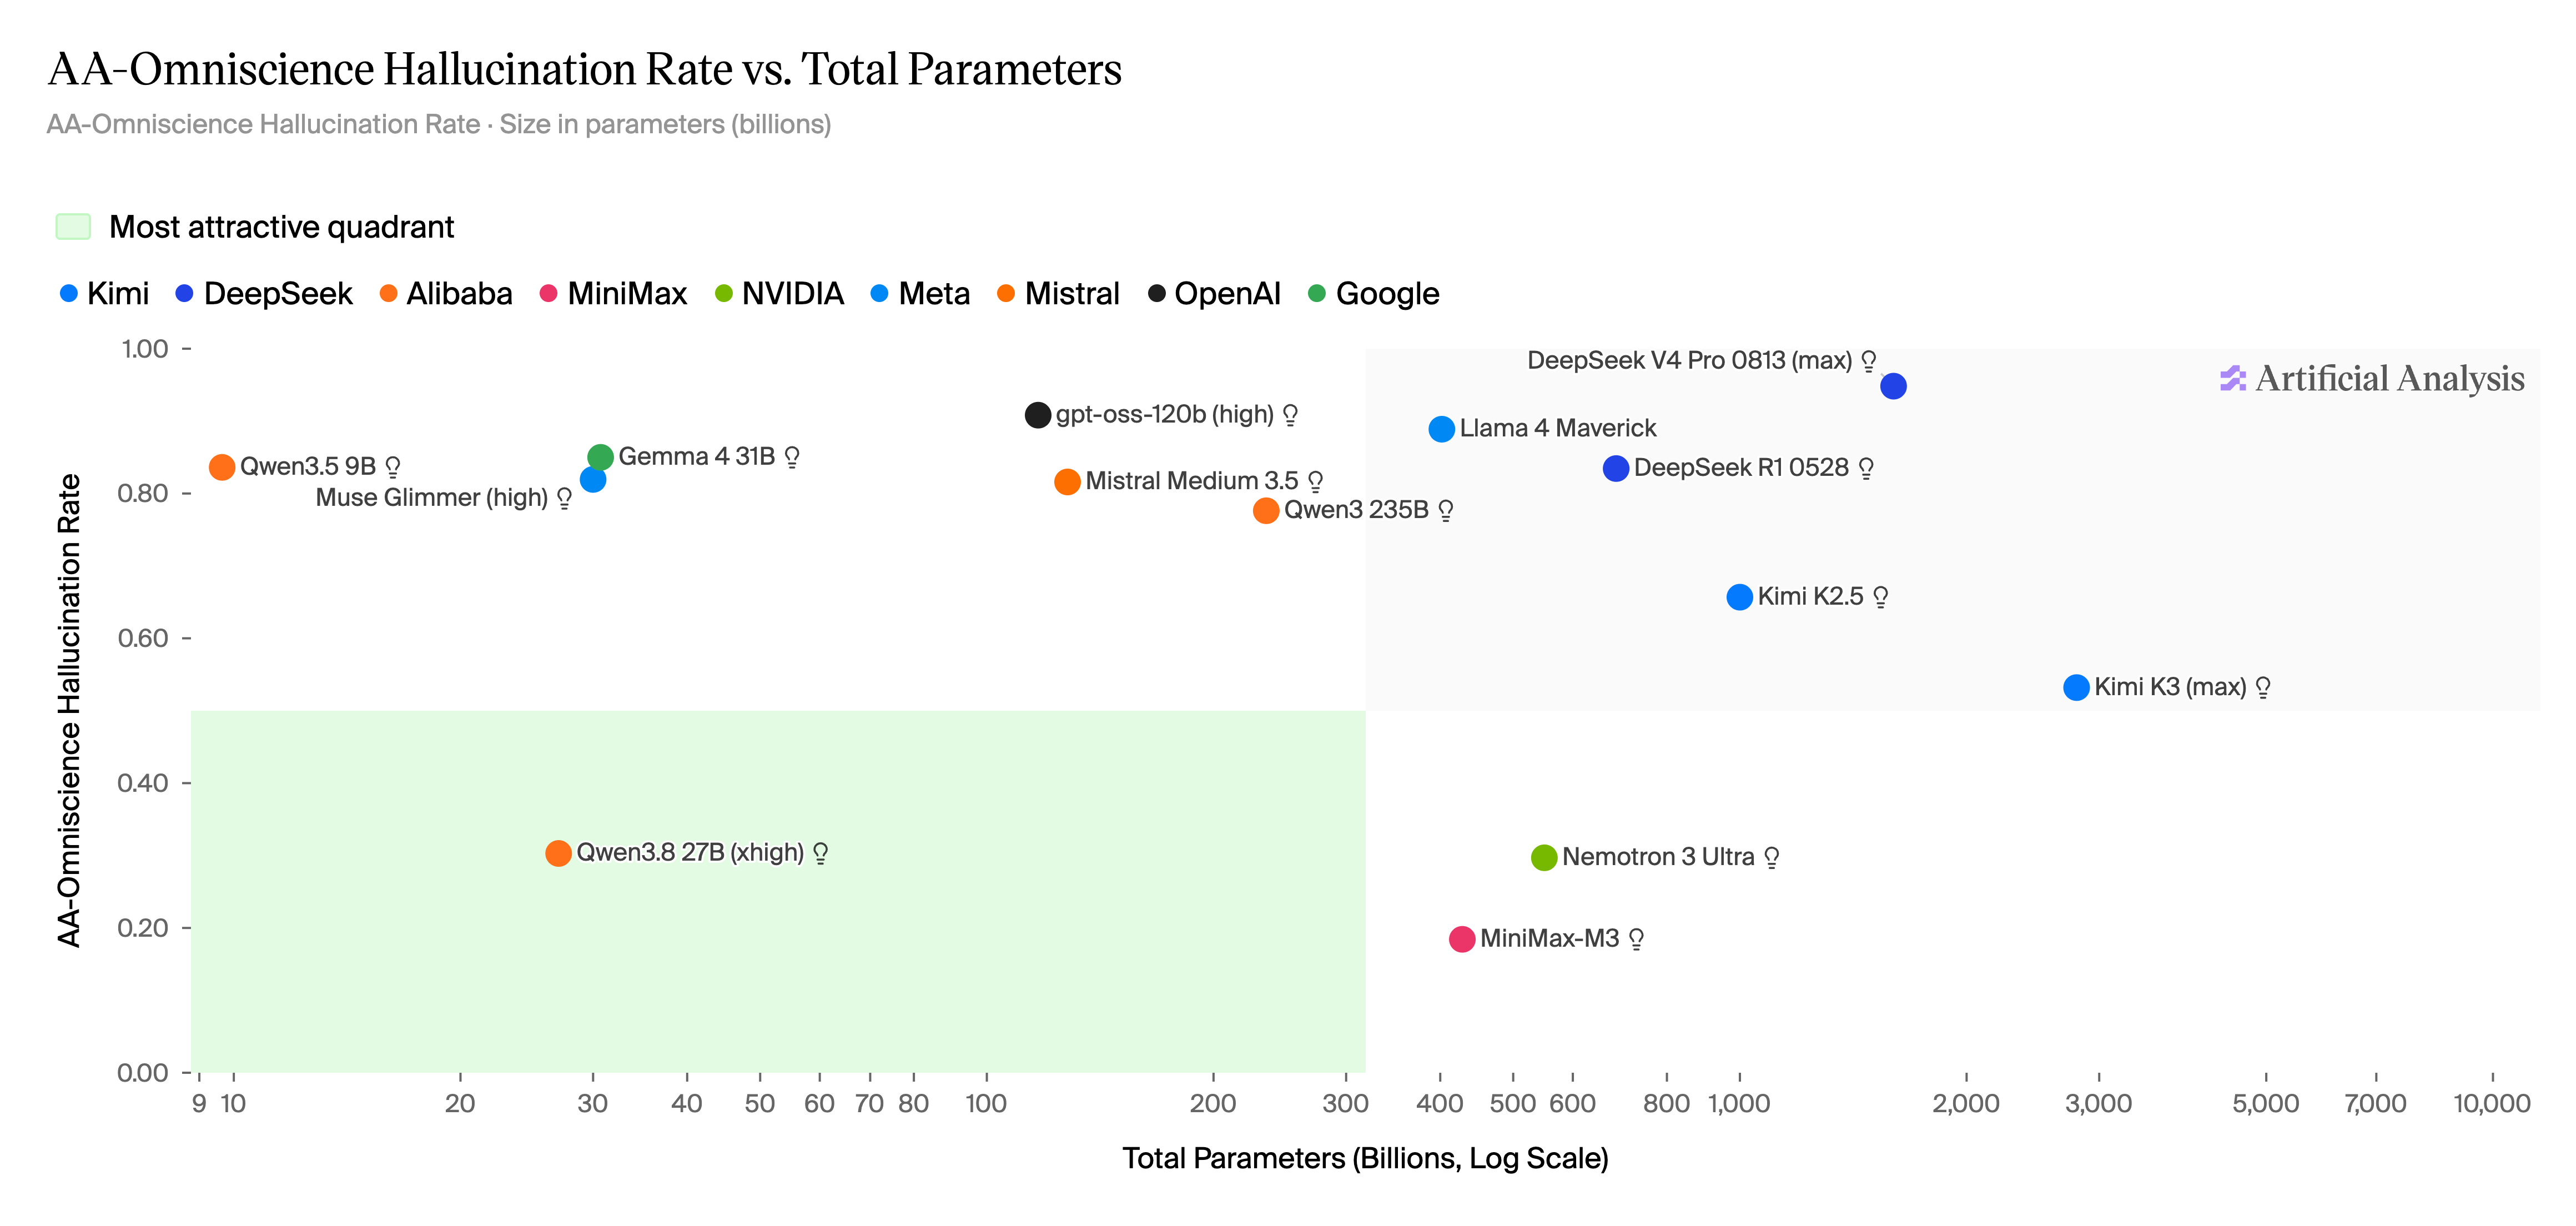
\includegraphics[width=0.98\linewidth]{figures/AA-Omniscience Hallucination Rate vs- Total Parameters (26 Aug '26) (1).png}}{\fbox{\parbox{0.90\linewidth}{\textbf{Source graphic not supplied.} Restore the original AA-Omniscience snapshot image from the source project. No measurements are reconstructed here.}}}
\par\smallskip
\IfFileExists{figures/AA-Omniscience Index - Score vs- Release Date (26 Aug '26).png}{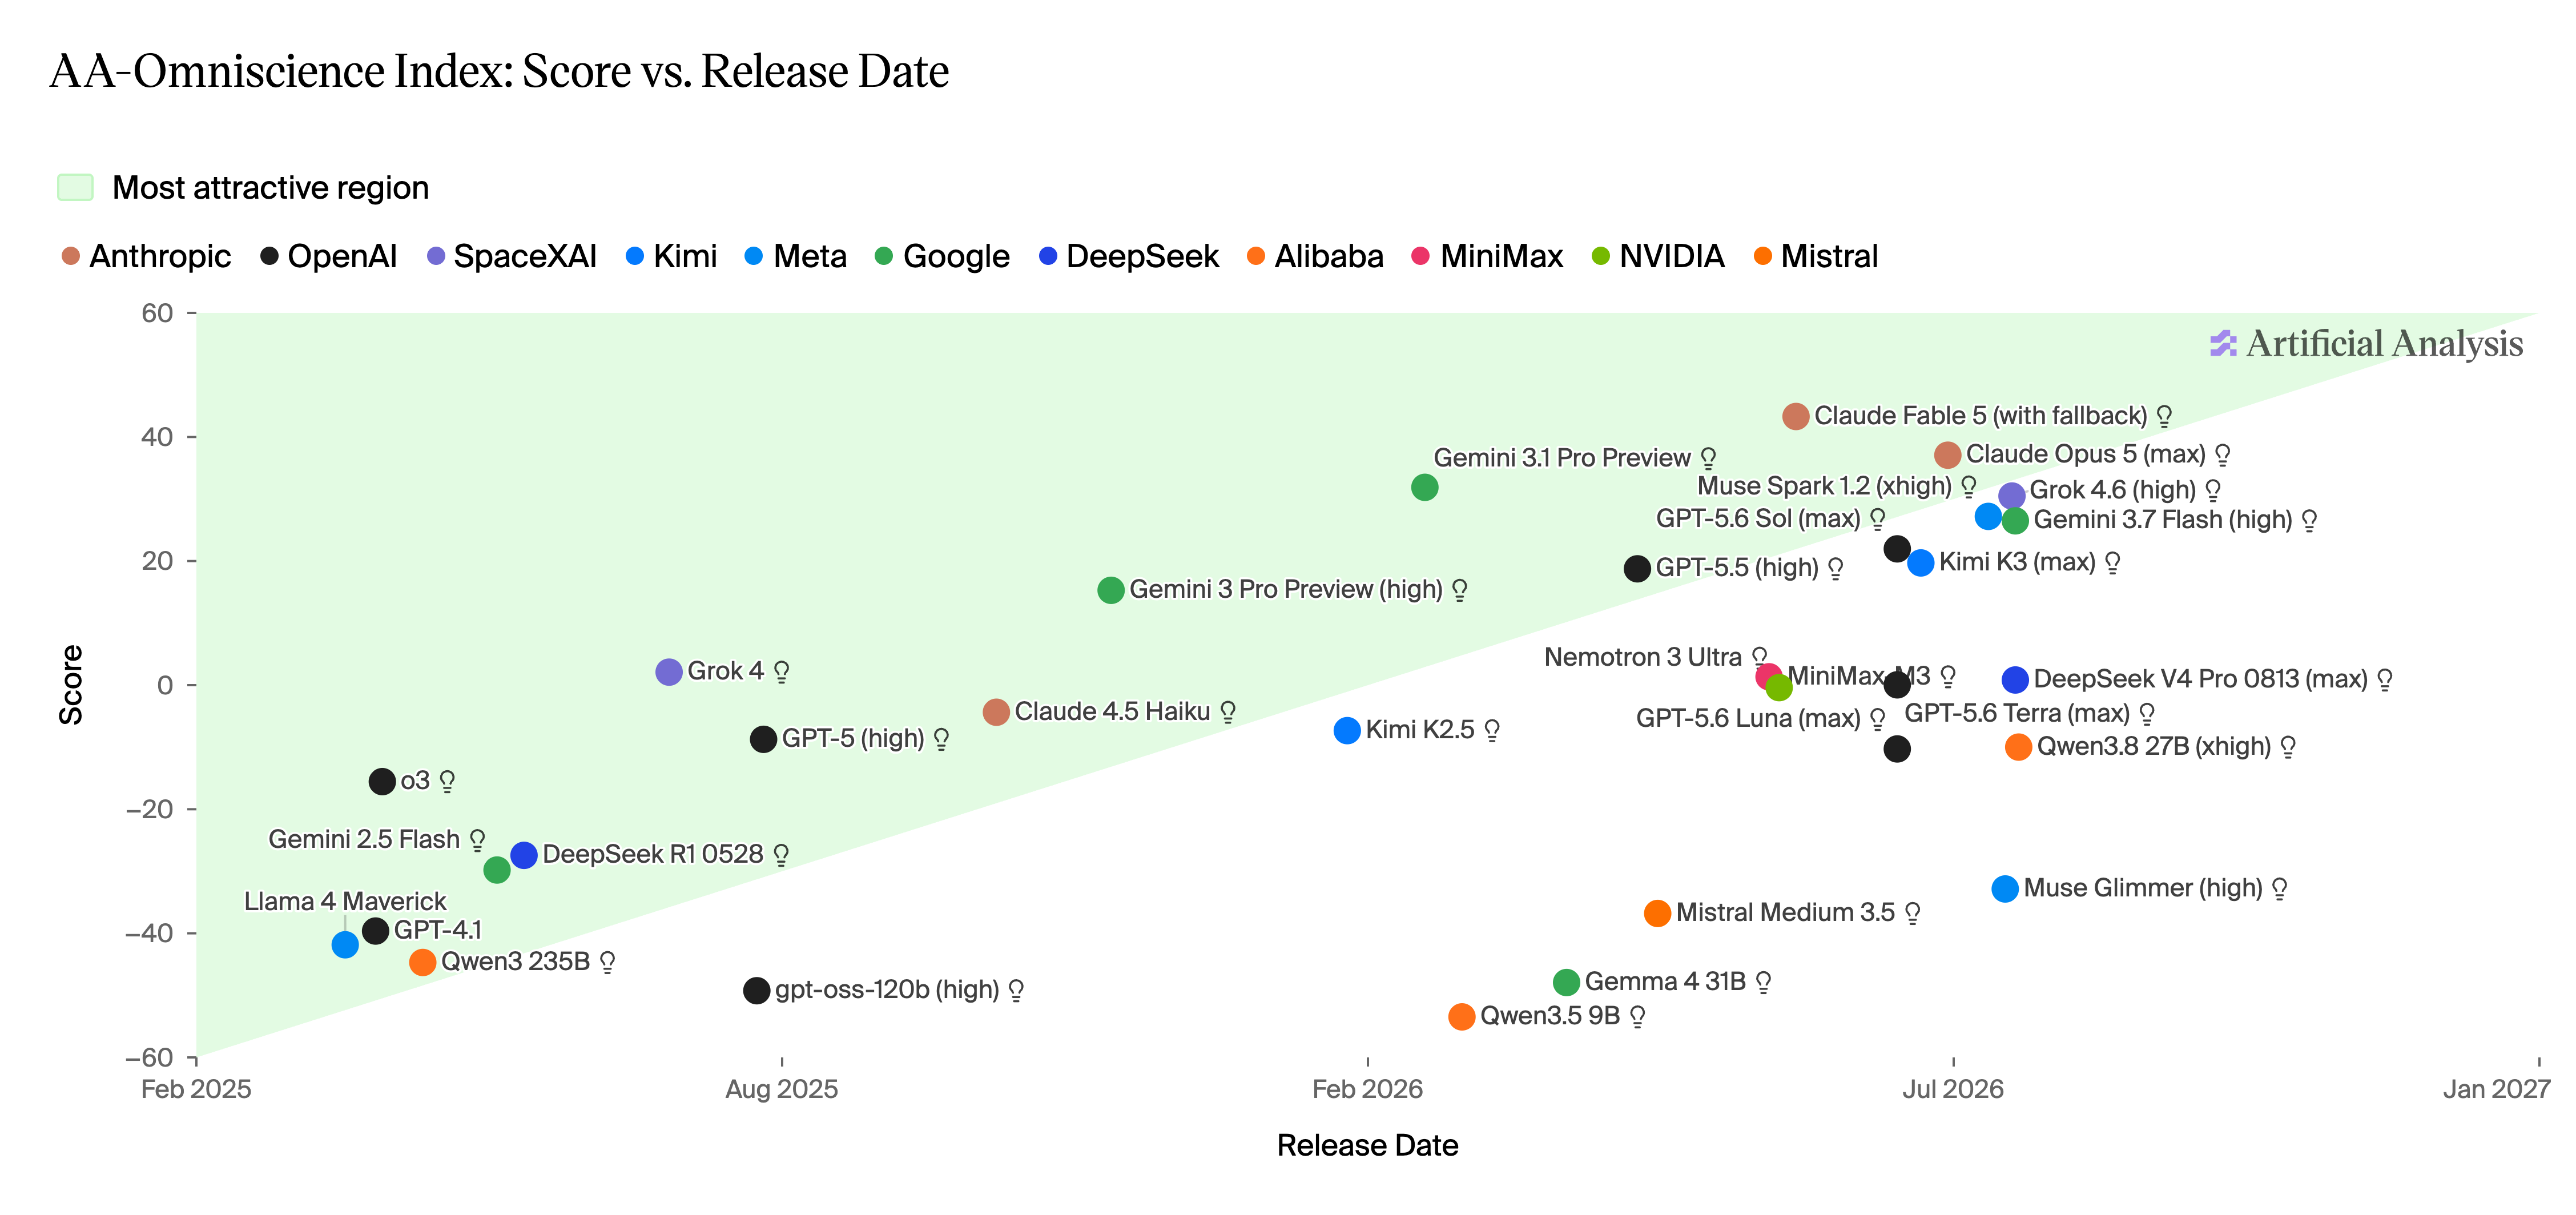
\includegraphics[width=0.98\linewidth]{figures/AA-Omniscience Index - Score vs- Release Date (26 Aug '26).png}}{\fbox{\parbox{0.90\linewidth}{\textbf{Source graphic not supplied.} Restore the original AA-Omniscience snapshot image from the source project. No measurements are reconstructed here.}}}
\caption{\textbf{AA-Omniscience leaderboard snapshot, August 26, 2026.}
Top: AA-Omniscience hallucination rate versus disclosed total parameters for
selected open-weight model configurations (lower is better; logarithmic
$x$-axis). Bottom: Omniscience Index versus release date for selected model
configurations (higher is better). The panels compare different models at one
date; they do not track one model family over time or isolate the effect of
model size. Source and graphics: Artificial Analysis
\citep{artificialanalysis_omniscience_leaderboard_2026}.}
\label{fig:aa-omniscience-snapshot}
\end{figure}

The plotted models differ in their developers, architecture, training,
post-training, and inference settings. The parameter panel includes only
models with a disclosed total parameter count. The release-date panel does
not hold these other choices fixed, and the leaderboard's grader and
methodology changed between the 2025 launch analysis and this snapshot.
The figures therefore cannot establish a causal relation between size or
release date and reliability, or prove that hallucination never decreases.
They provide descriptive context for Section~\ref{subsec:relative}, not
evidence that truth-contract evaluation works better than other methods.

\clearpage
\bibliography{references}

\end{document}
